\documentclass[11pt,a4paper,twoside]{article}

% Deutsche Spracheinstellungen
\usepackage[english,english]{babel, varioref}
\usepackage[T1]{fontenc}
\usepackage[utf8]{inputenc}

%\usepackage{marvosym}

\usepackage{amsfonts}
\usepackage{amssymb}
\usepackage{amsmath}
\usepackage{amscd}
\usepackage{amstext}
\usepackage{float}
\usepackage{caption}
\usepackage{wrapfig}
\usepackage{setspace}
%\usepackage[onehalfspacing]{setspace}
\usepackage{threeparttable}
\usepackage{footnote}
\usepackage{feynmf}
\usepackage{bbm}
\usepackage{slashed}
\usepackage{textcomp}
\usepackage{multirow}
\usepackage{courier}
\usepackage{listings}
\usepackage{color}
%\usepackage{minipage}
 
 \definecolor{middlegray}{rgb}{0.5,0.5,0.5}
 \definecolor{lightgray}{rgb}{0.8,0.8,0.8}
 \definecolor{orange}{rgb}{0.8,0.3,0.3}
 \definecolor{yac}{rgb}{0.6,0.6,0.1}
 \definecolor{puple}{rgb}{0.62,0.12,0.94}
 \lstset{language=Python,
                basicstyle=\ttfamily,
                keywordstyle=\color{red}\ttfamily,
                stringstyle=\color{magenta}\ttfamily,
                commentstyle=\color{blue}\ttfamily,
                morecomment=[l][\color{blue}]{\#},
		%stepnumber=1,
		%numberstyle=\color{magenta}\ttfamily,
		%    numbers=left,
		%    numberstyle={},
		%    numberblanklines=false,
		%    stepnumber=1,
		%    numbersep=10pt,
		    xleftmargin=15pt,
 		moredelim=[is][\color{purple}]{|}{|}
}

\newfloat{formel}{htbp}{for}
\floatname{formel}{Formel}

\onehalfspacing
%\setstretch {1.433}

\usepackage{longtable}

%\usepackage{bibgerm}

\usepackage{footnpag}

\usepackage{ifthen}                 %%% package for conditionals in TeX
\usepackage[amssymb]{SIunits}
%Fr textumflossene Bilder und Tablellen
%\usepackage{floatflt} - veraltet

%Fr Testzwecke aktivieren, zeigt labels und refs im Text an.
%\usepackage{showkeys}

% Abstand zwischen zwei Abs�zen nach DIN (1,5 Zeilen)
% \setlength{\parskip}{1.5ex}

% Einrckung am Anfang eines neuen Absatzes nach DIN (keine)
%\setlength{\parindent}{0pt}

% R�der definieren
% \setlength{\oddsidemargin}{0.3cm}
% \setlength{\textwidth}{15.6cm}

% bessere Bildunterschriften
\usepackage{caption2}


% Probleml�ungen beim Umgang mit Gleitumgebungen
\usepackage{float}

% Nummeriert bis zur Strukturstufe 3 (also <section>, <subsection> und <subsubsection>)
%\setcounter{secnumdepth}{3}

% Fhrt das Inhaltsverzeichnis bis zur Strukturstufe 3
%\setcounter{tocdepth}{3}

\usepackage{exscale}

\newenvironment{dsm} {\begin{displaymath}} {\end{displaymath}}
\newenvironment{vars} {\begin{center}\scriptsize} {\normalsize \end{center}}


\newcommand {\en} {\varepsilon_0}               % Epsilon-Null aus der Elektrodynamik
\newcommand {\lap} {\; \mathbf{\Delta}}         % Laplace-Operator
\newcommand {\R} { \mathbb{R} }                 % Menge der reellen Zahlen
\newcommand {\e} { \ \mathbf{e} }               % Eulersche Zahl
\renewcommand {\i} { \mathbf{i} }               % komplexe Zahl i
\newcommand {\N} { \mathbb{N} }                 % Menge der nat. Zahlen
\newcommand {\C} { \mathbb{C} }                 % Menge der kompl. Zahlen
\newcommand {\Z} { \mathbb{Z} }                 % Menge der kompl. Zahlen
\newcommand {\limi}[1]{\lim_{#1 \rightarrow \infty}} % Limes unendlich
\newcommand {\sumi}[1]{\sum_{#1=0}^\infty}
\newcommand {\rot} {\; \mathrm{rot} \,}         % Rotation
\newcommand {\grad} {\; \mathrm{grad} \,}       % Gradient
\newcommand {\dive} {\; \mathrm{div} \,}        % Divergenz
\newcommand {\dx} {\; \mathrm{d} }              % Differential d
\newcommand {\cotanh} {\; \mathrm{cotanh} \,}   %Cotangenshyperbolicus
\newcommand {\asinh} {\; \mathrm{areasinh} \,}  %Area-Sinus-Hyp.
\newcommand {\acosh} {\; \mathrm{areacosh} \,}  %Area-Cosinus-H.
\newcommand {\atanh} {\; \mathrm{areatanh} \,}  %Area Tangens-H.
\newcommand {\acoth} {\; \mathrm{areacoth} \,}  % Area-cotangens
\newcommand {\Sp} {\; \mathrm{Sp} \,}
\newcommand {\mbe} {\stackrel{\text{!}}{=}}     %Must Be Equal
\newcommand{\qed} { \hfill $\square$\\}
\newcommand{\midtilde}{\raisebox{-0,25\baselineskip}{\textasciitilde}}
\renewcommand{\i} {\imath}
\def\captionsngerman{\def\figurename{\textbf{Abb.}}}

%%%%%%%%%%%%%%%%%%%%%%%%%%%%%%%%%%%%%%%%%%%%%%%%%%%%%%%%%%%%%%%%%%%%%%%%%%%%
% SWITCH FOR PDFLATEX or LATEX
%%%%%%%%%%%%%%%%%%%%%%%%%%%%%%%%%%%%%%%%%%%%%%%%%%%%%%%%%%%%%%%%%%%%%%%%%%%%
%%%
\ifx\pdfoutput\undefined %%%%%%%%%%%%%%%%%%%%%%%%%%%%%%%%%%%%%%%%% LATEX %%%
%%%
\usepackage[dvips]{graphicx}       %%% graphics for dvips
\DeclareGraphicsExtensions{.eps,.ps}   %%% standard extension for included graphics
\usepackage[ps2pdf]{thumbpdf}      %%% thumbnails for ps2pdf
\usepackage[ps2pdf,                %%% hyper-references for ps2pdf
bookmarks=true,%                   %%% generate bookmarks ...
bookmarksnumbered=true,%           %%% ... with numbers
hypertexnames=false,%              %%% needed for correct links to figures !!!
breaklinks=true,%                  %%% breaks lines, but links are very small
linkbordercolor={0 0 1},%          %%% blue frames around links
pdfborder={0 0 112.0}]{hyperref}%  %%% border-width of frames
%                                      will be multiplied with 0.009 by ps2pdf
%
\hypersetup{ pdfauthor   = {Dimitrios Skodras},
pdftitle    = {Fermionic Dark Matter and its Role on B Anomalies}, pdfsubject  = {masterthesis}, pdfkeywords = {dark matter},
pdfcreator  = {LaTeX with hyperref package}, pdfproducer = {dvips
+ ps2pdf} }
%%%
\else %%%%%%%%%%%%%%%%%%%%%%%%%%%%%%%%%%%%%%%%%%%%%%%%%%%%%%%%%% PDFLATEX %%%
%%%
\usepackage[pdftex]{graphicx}      %%% graphics for pdfLaTeX
\DeclareGraphicsExtensions{.pdf}   %%% standard extension for included graphics
\usepackage[pdftex]{thumbpdf}      %%% thumbnails for pdflatex
\usepackage[pdftex,                %%% hyper-references for pdflatex
bookmarks=true,%                   %%% generate bookmarks ...
bookmarksnumbered=true,%           %%% ... with numbers
hypertexnames=false,%              %%% needed for correct links to figures !!!
breaklinks=true,%                  %%% break links if exceeding a single line
linkbordercolor={0 0 1},
linktocpage]{hyperref} %%% blue frames around links
%                                  %%% pdfborder={0 0 1} is the default
\hypersetup{
pdftitle    = {Fermionic Dark Matter and its Role on B Anomalies}, %right place
pdfsubject  = {master thesis}, 
pdfkeywords = {V301, Innenwiderstand, Leistungsanpassung},
pdfsubject  = {Protokoll AP},
pdfkeywords = {V301, Innenwiderstand, Leistungsanpassung}}
%                                  %%% pdfcreator, pdfproducer,
%                                      and CreationDate are automatically set
%                                      by pdflatex !!!
\pdfadjustspacing=1                %%% force LaTeX-like character spacing
\usepackage{epstopdf}
%
\fi %%%%%%%%%%%%%%%%%%%%%%%%%%%%%%%%%%%%%%%%%%%%%%%%%%% END OF CONDITION %%%
%%%%%%%%%%%%%%%%%%%%%%%%%%%%%%%%%%%%%%%%%%%%%%%%%%%%%%%%%%%%%%%%%%%%%%%%%%%%
% seitliche Tabellen und Abbildungen
%\usepackage{rotating}
\usepackage{ae}
\usepackage{
  array,
  booktabs,
  dcolumn
}
\makeatletter 
  \renewenvironment{figure}[1][] {% 
    \ifthenelse{\equal{#1}{}}{% 
      \@float{figure} 
    }{% 
      \@float{figure}[#1]% 
    }% 
    \centering 
  }{% 
    \end@float 
  } 
  \makeatother 


  \makeatletter 
  \renewenvironment{table}[1][] {% 
    \ifthenelse{\equal{#1}{}}{% 
      \@float{table} 
    }{% 
      \@float{table}[#1]% 
    }% 
    \centering 
  }{% 
    \end@float 
  } 
  \makeatother 
%\usepackage{listings}
%\lstloadlanguages{[Visual]Basic}
%\allowdisplaybreaks[1]
%\usepackage{hycap}
%\usepackage{fancyunits}

\usepackage{xfrac}
\usepackage{xcolor}
\usepackage{setspace}\usepackage{threeparttable}
\usepackage{fancyhdr}
\usepackage{graphicx}
\numberwithin{equation}{section}
%\usepackage{epstopdf}
\newcommand{\ti}{\text{i}}
\fancyfoot{}
\fancyhead[RO,LE]{\thepage}
\fancyhead[LO]{\leftmark}
\fancyhead[RE]{\rightmark}


 %\setlength{\parskip}{1.5ex}
\begin{document}
\begin{spacing}{1,2}
\pagenumbering{Roman}

% Anmerkung: Die Seitenraender wurden asymmetrisch gewaehlt,
%            damit genug Platz fuer eine Klemmbindung da ist.
%            Da neue Kapitel auf der rechten Seite (ungerade
%            Seitennummer) beginnen sollten, muss ggf. am Ende
%            des vorhergehenden Kapitels eine Leerseite
%            eingefuegt werden:
%
%            \newpage
%            \thispagestyle{empty}
%            \ \\
%            \newpage
%
%            Die Seitenraender koennen aber auch in der Datei Tex/global.tex
%            veraendert werden.

% >>> Titelseite <<<

\newcommand{\thetitle}{Majorana Dark Matter and its Role in B-anomalies}

\thispagestyle{empty}
\begin{center}

\Huge\textbf{\thetitle}
\vfill
% Note that the size is given in normal parentheses
% instead of curly brackets.
% Define external vertices from bottom to top
\vfill
\Large
Masterarbeit\\ zur Erlangung des akademischen Grades \\ Master of Science \\
\vspace{20pt}
\normalsize
vorgelegt von \\[5pt]
{\Large Dimitrios Skodras} \\[5pt]
geboren in Aschaffenburg \\
\vspace{20pt}
Lehrstuhl für Theoretische Physik IV \\ Fakultät Physik \\
Technische Universität Dortmund \\ 2016
\end{center}
\newpage
% % >>> Gutachterseite <<<
% \thispagestyle{empty}
% \newpage
% \cleardoublepage

\thispagestyle{empty}
\vspace*{\fill}
\begin{tabbing}
1. Gutachter : \=\kill
1. Gutachter : \>Prof. Dr. Gudrun Hiller \\[11pt]
2. Gutachter : \>Prof. Dr. Jean Orloff \\[11pt]
\end{tabbing}
\vspace{11pt}
Datum des Einreichens der Arbeit: 31. Oktober, 2016
\newpage
\thispagestyle{empty}
\begin{flushright} 
\textit{\grqq Es gibt nichts Praktischeres, als eine gute Theorie.\grqq}\\
- \textit{Kant, Immanuel}\\
\vspace{2cm}
% \textit{``Was dürfen wir hoffen?''}\\
% - \textit{Kant, Immanuel}\\
% \vspace{2cm}
% \textit{``Kein Mensch ist so wichtig, wie er sich nimmt.''}\\
% - \textit{Kant, Immanuel}
\end{flushright}

\newpage


% >>> Kurzfassung/Abstract <<<

\thispagestyle{empty}
%Kuzfassung
 \section*{Kurzfassung}

 \section*{Abstract}

 \section*{Abrégé}
 \newpage

% >>> Hauptteil <<<

%\addcontentsline{toc}{chapter}{Inhaltsverzeichnis}
\end{spacing}
\begin{spacing}{1,1}
\tableofcontents\newpage

\end{spacing}
\begin{spacing}{1,2}

\thispagestyle{empty}
 \cleardoublepage

\pagenumbering{arabic}
\setcounter{page}{1}
\pagestyle{fancy}

\section{Introduction}
After the prediction (1964) (CITE) and the experimental verification (2012) (CITE) of the
now called Higgs-boson, the Standard Model (SM) could be considered self-
contained. The forecasts it makes for processes described therein are proven
remarkably well by various experiments. At least at the energy scales they
are currently operating. That said, it already contains associations that the
contributions to this magnificent theory, made by our scientific forefathers, might not be
the end of the story. We might know the Higgs mechanism being source of mass of visible particles,
but the reason for their absolute values is still notional. The fermions thereof can be put into
small groups and are considered to be interacting equally with the gauge bosons but it appears
that some break ranks. Not only in the elementary particle physics sphere but also in cosmology
strange things happen. From observation it seems that there has to be a mass distribution of
invisible particles, say dark matter, that lead to the actual orbits of the stars in the galaxy.
There is of course even more, but the resolution of these three issues in one combined theory is
the task of this thesis.

\noindent To resolve a problem, one has to understand it first. So we start with some notes on 
related topics in the SM and cosmology.


% It still lacks for example a quantum field theoretical
% description for gravity or does not contain the experimentally shown masses
% of the neutrinos. Besides, its dynamics depend on 19 parameters, including
% the masses of the fermions, which are quite a lot and are wanted to decrease
% in number by finding relations among one another. Furthermore cosmology
% tells us that the SM is only covering about twenty per cent of the mass content
% of the universe where the rest is made of the nowadays called dark matter
% (DM). Since this thesis is about flavour and dark matter, we
% should have a closer look on the way things stand at the moment.


\section{A Guide to today's Physics}

\subsection{Flavour in the SM}
% The Standard Model is a theory that contains particle fields, ordinary matter is composed of and messenger fields mediating interactions between them. 
% These fields can be separated by their quantum numbers indicating their couplings to each other. At first we have the twelve gauge vector boson fields, 
% eight gluon fields $G_a$ for strong interactions with coloured ($C$) particles and four electroweak boson fields $W_1$, $W_2$, $W_3$ and $B$ which couple
% to particles with weak isospin $T$ and hypercharge $Y_W$ respectively. Now we have 24 fermion fields, six leptons and six quarks each carrying one of three colours.
% The leptons can be subdivided into three electrically ($Q=T+Y_W$) charged and three uncharged ones and the quarks into three up-type ($T=\sfrac12$) and
% three down-type ($T=-\sfrac12$). Last but not least, the already mentioned scalar Higgs-field $\phi$ which develops a non vanishing vacuum expectation value
% (vev) $v$. This is the source for the spontanious breaking of the electroweak symmetry into the electromagnetic 
% (NOT)
The Standard Model is a gauge quantum field theory whose internal symmetry is the unitary product group $SU(3)_C\times SU(2)_L\times U(1)_{Y_W}$ representing
the quantum chromodynamics (QCD) whose charge is called color $C$ and the electroweak theory (GSW-Theory) whose charges are the weak isospin $T$ 
(hold by left handed particles) and the weak hypercharge $Y_W$. These quantum numbers (QN) are carried by a set of particle fields, ordinary matter is composed
of and messenger fields mediating these interactions between them. In particular twelve gauge vector boson fields, eight gluon fields $G_a$ for strong 
interactions and four electroweak boson fields from which $W_1$, $W_2$, $W_3$ couple to the weak isospin and $B$ to the weak hypercharge. Now we have 12
fermion fields, six leptons $e$, $\mu$, $\tau$ as well as their respective neutrinos $\nu$ and six quarks $u$, $d$, $s$, $c$, $b$, and $t$. Actually there
are even more since they are defined by their QN. So for each fermion there is a distinction drawn between left handed $f_L$ ($T=\sfrac12$) and right 
handed $f_R$ ($T=0$), although $\nu_R$ are not considered in the SM. Furthermore there are three different colours for each quark. Well finally the field 
$\phi$ of the already mentioned scalar
Higgs-boson holds a special role in the SM. It is known that the boson fields $W^\pm$ and $Z$, responsible for weak processes, have nonzero masses. But their
mass terms would break the gauge invariance of the lagrangian. So the Higgs-mechanism was considered wherein $\phi$ develops a non vanishing vacuum expectation
value $v$ (vev) which breaks the electroweak symmetry spontaniously down to the electromagnetic symmetry $U(1)_Q$ resulting in a still massless photon field 
$A$ and the three just named massive ones.
\subsubsection{Yukawa Interaction}
Not only the bosons get their masses from this mechanism but the fermions as well - at least the electrically charged ($Q$) ones - which is represented by the
Yukawa (scalar-fermion interaction) term in the SM-lagrangian
\begin{equation}
 \mathcal{L}_{Y} = - y^u_{ij}\, \bar Q^i_L \, \phi^c\, u^j_R - y^d_{ij}\, \bar Q^i_L\, \phi\, d^j_R - y^e_{ij}\, \bar L^i_L\, \phi\, e^j_R + \text{h.c.}.
 \label{eq_yukawaSM}
\end{equation}
\noindent
$y^u$, $y^d$ and $y^e$ are $3\times 3$ (three generations) real, so called yukawa matrices and represent the 
coupling of the fermions to the Higgs. $\phi^c = \ti\sigma_2\phi^*$ is the charged conjugate Higgs. ``h.c.'' stands for hermetian conjugate so that it holds for the antiparticles as well. 
$Q_L$, $L_L$ and $\phi$ are doublets of the $SU(2)_L$, since they are built out of two fermion fields each holding a 
weak isospin of $T=\sfrac12$ with the 3rd component $T_3 = \pm\sfrac12$, e.g. $L^2_L = (\nu_{\mu\, L}, \mu_L)^T_{\textbf{2}}$ with the left handed muon-neutrino and the muon. 
Their counterparts $u_R$, $d_R$ and $e_R$ are singlets under the $SU(2)_L$ because they have no weak isospin, e.g. $e^2_R = (\mu_R)_{\textbf{1}}$, and hence don't take part
in the weak interaction mediated by the $W$-bosons. After 
the symmetry breaking and rotating the fermion fields in a basis where the yukawa matrices become diagonal, we can write down their mass terms 
\begin{equation}
 \mathcal{L}_m = -m^u_i \bar u'^i_L u'^i_R -m^d_i \bar d'^i_L d'^i_R -m^e_i \bar e'^i_L e'^i_R 
 \label{eq_massSM}
\end{equation}
\noindent
where $m^\alpha_i \sim y^\alpha_i \cdot v$ ($\alpha = u,d,e$). Here you can see that the SM does not distinguish between generations. 
It treats a left handed up quark the same way it treats a left handed charm or a left handed top. So if the eigenvalues of $m^\alpha$ would be degenerate, i.e. the masses would
be all the same, one would not have a method to differentiate them. 

% \vspace{-0.3cm}
You could ask
what happened with a term like $\nu_R$ in \eqref{eq_yukawaSM}. This would imply a particle which has neither a color charge, nor electrical charge, nor 
weak isospin and hence ($Q = T_3 + Y_W$) no hypercharge which means that the SM is totally blind to it. Furthermore it seemed obvious not to be
able to construct a neutrino mass since they were considered massless. But to answer the question we could add 
such a term somehow when it can be shown for example that righthanded neutrinos exist, which is likely due to the measurements of neutrino oscillations.



\subsubsection{Weak Interaction}
Neutrino oscillation is a process where a neutrino of one generation changes its flavour while propagating through space described by the PMNS matrix. 
This suggests that 
flavour is not a conserved quantum number in nature unlike the electrical charge for example. As this phenomenon is still rather young (2001) and not implemented in the 
SM, we already have flavour violation (FV) therein, in the quark sector. There is a huge list of Mesons and Baryons (composites of one quark and one anti-quark,
or three quarks, respectively) decaying into others with different quark content enabled by the $W$-bosons via charged currents. 
\\ \\ \textit{Flavour Changing Charged Currents}\\
\noindent So it was thought, that the down-type quark mass
eigenstates $d'^i$ are superpositions of their interaction eigenstates $d^i$. Formerly started by Cabibbo and pursued by 
Kobayashi and Maskawa (1973) for CP-violation reasons (charge conjugation C, parity P), the CKM-matrix as an unitary $3\times 3$ matrix was invented,
which can be thought of as a rotation
matrix, rotating the weak eigenstates of the down-type quarks in the mass eigenstates by three Euler angles, $\theta_{12} = \theta_C$ called Cabibbo angle 
as well as $\theta_{23}$ and $\theta_{13}$.
\begin{equation}
 \begin{pmatrix}
  d' \\ s' \\ b'
 \end{pmatrix} = V_\text{CKM}  \begin{pmatrix}
  d \\ s \\ b
 \end{pmatrix},
\end{equation}
\noindent
where $V_\text{CKM}$ can be parameterised by $\lambda = \sin(\theta_C) \approx 0.2$ at leading order (LO) as
\begin{equation}
 V_\text{CKM} \approx \begin{pmatrix}
  1 & \lambda & \lambda^3\\
  -\lambda & 1 & \lambda^2\\
  -\lambda^3 & -\lambda^2 & 1
 \end{pmatrix}.
\end{equation}
The up-type quarks have no differences between their weak and mass eigenstates, but we could have played the same game with them leading to the 
same mixing, since $V_\text{CKM}$ is unitary. Looking at this matrix one can see that it is almost diagonal and hierachical which
means that the farther you leave the main diagonal the smaller become the magnitudes of the entries. It can be asked 
\\ \\ \textit{Flavour Changing Neutral Currents}\\
\noindent TO REVISE!
One problem of Cabibbo's theory is that a process $d'\bar {d'} \rightarrow Z$ would lead to an FCNC at tree level but is in fact highly suppressed. This
could be explained by the GIM-mechanism 


Now comes one of the basic questions motivating this thesis: Are these patterns random or is there rather an underlying broken family-symmetry which
could serve as a blindman's stick for the SM? We go with our guts and prefer the latter suggestion.


\subsubsection{Flavour Anomalies}
\label{sec_flAnom}
\textit{Anomalous magnetic moment of the muon}\\
\noindent
In general, every charged particle
may have a spin $\boldsymbol{s}$ with an associated magnetic moment \cite{anomMom}
\begin{align}
 \boldsymbol{\mu} = g \frac{e}{2m}\boldsymbol{s}.
\end{align}
The factor $g$ is called the gyromagnetic factor and is equal for all elementary particles of a kind. For fermions it is $g=2$. By saying, the magnetic 
moment is anomalous, one states a deviation from this value which is expressed as $a= (g-2)/2$. There are many contributions to this already within the SM
from QED or hadronic vacuum polarisation which cause most of the uncertainties \cite{160606861} but all of them are quantum loop effects. Even when all of them are taken into account, there is still a discrepancy
between theory and experiment 
\begin{align}
 \Delta a_\mu = a_\mu^\text{ex} - a_\mu^\text{SM} = 287(80)\cdot 10^{-11}.
\end{align}
Contributions to $a$ can be evaluated in the following way. An ingoing muon with momentum $p_1$ radiates a photon $A_\mu (q)$, leaving the muon in the final 
state with $p_2$. To first order in the external field, the scattering amplitude is 
\begin{align}
 M = -\ti e \langle \mu_2|J^\mu(x=0)|\mu_1\rangle A_\mu(q),
\end{align}
with the electic current $J^\mu(x)$. The most general parametrisation one can write thanks to Ward identity and parity conservation in QED is for on-shell
($p_i^2 = m_i^2$) external muons
\begin{align}
 \langle \mu_2|J^\mu(0)|\mu_1\rangle = \bar u_2 \left[F_D(q^2)\gamma^\mu + F_P(q^2)\frac{\ti \sigma^{\mu\nu}q_\nu}{2m}\right] u_1.
 \label{eq_gordon}
\end{align}
In the non-relativistic limit, the relation between the magnetic moment and these form factors $F_D$ and $F_P$ can be derived to be
\begin{align}
 \mu = \frac{e}{2m}\left(F_D(0) + F_P(0)\right)
\end{align}
\noindent
with $F_D(0)=1$ but $F_P(0)\neq0$.
\\ \\ \textit{Semileptonic four-fermion operators}\\
Wilson Coefficient \cite{150306199}
\begin{align}
 C_9^\text{NP} = -C_{10}^\text{NP} \in [-0.71,-0.35]\quad \text{(at 1}\sigma),\\
 C_9^\text{NP} = -C_{10}^\text{NP} \in [-0.91,-0.18]\quad \text{(at 2}\sigma),
\end{align}
\\ \\ \textit{Four quark operators}\\
Bag parameter \cite{1607.00299}
\begin{align}
 B_{B_q}(\mu) = \frac{3}{8f_{B_q}^2 m_B^2} \langle \bar B_q |O_q|B_q \rangle
\end{align}
Mass difference \cite{1102.0009}
\begin{align}
 \Delta m_q \propto f^2_{B_q} \hat{B}_{B_q}
\end{align}
Wilson Coefficient
\begin{align}
 \frac{\Delta m_s^\text{exp}}{\Delta m_s^\text{SM}}-1 = \frac{C_{B\bar B}}{C^\text{SM}_{B\bar B}}
\end{align}
with $\Delta m_s^\text{exp} = 1.1688(14) \cdot 10^{-11}$ GeV (PDG) \cite{1602.03560} and $\Delta m_s^\text{SM} = 1.332(213)\cdot 10^{-11}$ GeV \cite{0612167}%\cite{1102.0009}
and $C_{B\bar B}^\text{SM} \simeq 8.2\cdot 10^{-5}$ TeV$^{-2}$ 
\begin{align}
 C_{BB} \in [-2.0,0.3] \cdot 10^{-5} \text{TeV}^{-2}.%\quad \text{(at 2}\sigma).
\end{align}
\\ \\ \textit{Majorana}\\
\begin{equation}
\begin{aligned}
 \frac{C^{-1}\left(\slashed{k}+m\right)}{(k^2-m^2}\\
 \frac{\left(\slashed{k}+m\right)C}{k^2-m^2}
\end{aligned}
\label{eq_majoProp}
\end{equation}
\begin{equation}
\begin{aligned}
 w^c = \gamma_0 C w^*
 \bar {w^c}= w^T C^{-1}
\end{aligned}
\label{eq_ChargeConj}
\end{equation}
\cite{Fierz}
\begin{align}
 \left(u_{L,R}\right)^c = v_{R,L}
\end{align}





\subsubsection{Effective Field Theory}
\cite{BurasEFT} simple derivation of EFT in SM as 4-fermi. Extraction of Wilson coefficients.
To get such a
low energy theory, one uses the framework of the Operator Product Expansion (OPE)


\subsection{DM in the $\Lambda$-CDM}

From the smallest scales, we are heading to the largest in the universe. The effects happening there are discribed by the Big Bang cosmology, parameterised
by the $\Lambda$-CDM model. It was developped in the late 1990's \cite{LambdaCDM} to give an explanation for, among other things, the energy density of the 
universe. The model's name refers to the sources adjusting the lack of energy. The $\Lambda$ points to the cosmological constant in Einstein's field equation
in the context of general relativity which connects the curvature of space with the stress-energy tensor.
The CDM stands for cold dark matter, speaking particles moving slowly with respect to the speed of light (cold) and interacting very weakly with luminous
matter (dark). We now shortly present two hints for its existence
The reasons for its existence and possible candidates satisfying the ensuing properties will be reviewed as well as the possiblities to test them.\\
\\ \textit{A: Rotational Curves}\\
\noindent The motion of stars is mainly influenced by their gravitational interactions \cite{LectDMLis}. From Newton's gravitation law, their circular velocity 
is derived as
$v(r)\propto\sqrt{M/r}$ with the radial distance $r$ from the center and the enclosed mass $M$. For $r$ larger than the the galactic disc, $M$ should remain
constant and the velocity should drop $\propto r^{-1/2}$. But appearently (RubinFord,RobertsWhitehurst) it approximates a constant. One explanation for this
is the lack of generality in Newton's law for very small accelerations which means it could by modified (MoND), but is at least not able to 
explain the anomalous behaviour all by itself \cite{11015122}\cite{160607790} and needs the help of the second possibility. Namely a mass distribution even beyond the galactic
disc with $M(r)\propto r$ consisting of particles, or rather objects, which are not interacting electromagnetically. The rotation curves suggest a 
spherically symmetric ($\rho_\text{DM}\propto 1/r^2$) halo that also implies that this dark matter does not interact strongly with itself as the visible 
baryonic matter which collapses to the disc. To serve for this issue, the existence of DM is coherent but with this observation,its total amount in the 
universe cannot be extracted. It should be stressed that the mass distribution does not have to be created by just one particle species. Baryonic dark matter
and the SM neutrinos also (may) contribute. \\
\\ \textit{B: Cosmic Microwave Background}\\
\noindent The CMB is a major proof for the Big Bang theory. It emerged due to an effect called recombination. 
To this point, radiation, electrons and nucleons made up a plasma and the photons were scattering a lot off the actual free electrons. But then it was 
energetically favoured for the electrons and nucleons to build light elements and the density of free electrons decreased which lead eventually to the decoupling
of the photons, meaning that they could travel freely without interacting. This residual amount of radiation has a wavelength in the microwave scale and is
very isotropic and follows the spectrum of a black body \cite{DM-EvCaDo}. The observed anisotropics analysed by several CMB experiments 
(WMAP \cite{1212.5226}, ACBAR \cite{0303515}, CBI \cite{0205388}) lead to a discrepancy
between the abundance of baryons and matter. We will now review the computation of the relic abundance and afterwards the different detection types, most 
notably direct detection.



\subsubsection{Relic Abundance}
\label{sec_RD}
Relic density \cite{1303.5076}, \cite{1607.02475}
\begin{align}
 \Omega_\text{DM} h^2 = 0.11805 \approx \frac{10^{-26} \text{cm}^3 / \text{s}}{ \langle \sigma v \rangle_\text{Ann}}
\end{align}





\subsubsection{Detection Methods}
\textit{Direct Detection} \\
\begin{align}
 \sigma_\text{DD} = \sigma_\text{SI} + \sigma_\text{SD} = \frac{4}{\pi}\mu_N \left(|f_N|^2 + 3*|a_N|^2\right)
 \label{eq_th.sigma.dd}
\end{align}
\\ \textit{Indirect Detection} \\
\\ \textit{Collider Signatures}

\section{Group Theory and Flavour Symmetries}
\subsection{Group Invariance}
% symmetry breaking,representations
\subsection{$U(1)_\text{FN}$ and Continuous Groups}
\label{sec_FNGT}
 \textit{Lie-Groups}\\
\\ \textit{Clebsch Gordan coefficients} \\
\\ \textit{Froggat Nielsen-formalism}

\subsection{$A4$ and Discrete Groups}
\label{sec_A4GT}
\textit{General Properties}\\
% finite amount of representations; characters; 
 \begin{align}
  \sum m_n n^2 = N_G \quad groupelements\\
  \sum m_n = \#_{IRR} \quad C = Irred\,Reps\\
  \varphi:\, G\rightarrow \text{GL}(V)\\
  g\mapsto \varphi(g):\, V\rightarrow V\\
  \chi_D(g) = \text{tr}D(g)\\
  \sum_g \chi_\alpha(g)^*\chi_\beta(g) = N_G \delta_{\alpha\beta}\\
  \sum_\alpha \chi_\alpha(g)^*\chi_\alpha(h) = \frac{N_G}{n_g} \delta_{C_g C_h} \stackrel{\Lambda}{=} \langle \chi^\mu, \chi^\nu \rangle = \delta^{\mu\nu}\\
  \text{FS}(R) := \frac{1}{N_G} \sum_g \chi_R(g^2) =\begin{cases}
                                                     1, & \text{real}\\
                                                     0, & \text{complex}\\
                                                     -1, & \text{pseudoreal}\\
                                                    \end{cases}\\
  \mu(k) = \langle \chi_R \cdot \chi_{R'} , \chi_{R_k} \rangle \quad tensor product decomposition\\
 \end{align}
 \\ \\ \textit{$A_4\times Z_3$}\\
%  tetrahedron; link to $T'$ just because its nice; smallest group with $\boldsymbol{3}$; PMNS matrix; $\theta_{13}$
%  seperation of leptons and neutrinos

\section{Model Outline}
\textit{The Underlying Model}\\
\noindent Now that we know the actors on the stage, we can build a model trying to reveal their behaviour altogether. We will follow basically the model constructed
in \cite{Grip}. They build a renormalisable theory which generates the anomalies associated with the $b$ and the $\mu$ at loop level. To do so, they 
introduce two new scalar fields $\Phi_l$ and $\Phi_q$ and a single fermion field $\chi$ which couple to SM-fermions via Yukawa interactions. 
Their conditions to reduce the amount of possible charge assignments for them are 
\begin{enumerate}
 \item the preservation of the accidental symmetries as baryon and lepton number and the prevention of other sources of flavour violation.
 \item scalar couplings with the Higgs as $\Phi H H$ or $\Phi H H H$ which could modify the observed Higgs phenomenology should be prevented.
 \item the coloured particle, required by quark interaction, should be a scalar since it will have weaker bounds on its mass.
 \item a $U(1)$ symmetry only interacting non trivially on the BSM fields has the advantage that all NP flavour-violating processes are loop suppressed. And
 moreover the lightest NP state (LP) would be stable that should be uncolored and electrically neutral. 
 \item the dimension of $SU(2)_L$ of the NP irreducibles is less then five.
\end{enumerate}
With these constraints they reject some representations of $\chi$ and $\Phi_l$ which could lead to unwanted renormalisable interactions, but they state 
that their LP would not fit the relic density and/or the direct detection bounds through the Z-coupling, although the anomalies are 
well explained by the model. \\ \\
\noindent \textit{Charge assignment}\\ \noindent
The main feature of this thesis is the adding of a flavour group $\mathcal{G} = U(1)_\text{FN}\times A_4 \times Z_3$ \cite{FerA4}\cite{VarzTotMod}. 
It shall prohibit these dangerous interactions by charging the respective fields so that the representations themselves are again enabled. Besides this,
the flavour patterns and the correct DM phenomeology are obtained. 
The downside herein is the surrender of renormalisability. Since we expect that NP couples chirally and that the fits say that the 4 fermion operator 
$\bar b_L \gamma^\nu s_L \mu_L \gamma_\nu \mu_L$ is prefered, we consider $SU(2)_L$ representations of $\chi$ that yield invariance and wherein the lightest
state has a small or vanishing $T_3$ in order to reduce its coupling to the $Z$. This can be achieved in many ways depending on what you want to get in the end. Besides the focus on heavy quarks,
our interest is a special role for the muon in order to explain its anomalous magnetic moment and the discrepancy in $B_s\rightarrow \mu\mu$. 
To do so, we want $\Phi_l$ to only couple to muons which can be ensured by representing it suitably under $A_4$. 
\begin{table}[t]
 \begin{tabular}{c|c|c|c}
%$SU(3)_C\times SU(2)_L\times U(1)_{Y_W}$
  Field & $\mathcal{G}_\text{SM}$ & $A_4 \times U(1)_\text{FN} \times Z_3$ & $U(1)_{B'}\times U(1)_{L'}\times U(1)_\chi$\\
  \hline
  $Q^i_L$ & (3,2,$\frac16$) & (1,$a^i$,$\omega$) & ($\frac13$,0,0)\\
  $U^i_R$ & (3,1,$\frac23$) & (1,$b^i$,$\omega^2$)& ($\frac13$,0,0)\\
  $D^i_R$ & (3,1,$-\frac13$) & (1,$c^i$,$\omega^2$)& ($\frac13$,0,0)\\
  $L^i_L$ & (1,2,$-\frac12$) & (3,0,$\omega$)& (0,1,0)\\
  $E^i_R$ & (1,1,$-1$) & ($1 {^(} {'} {^,} '' {^)} $,$d^i$,$\omega^2$)& (0,1,0)\\
  $H$ & (1,2,$\frac12$) & (1,0,1)& (0,0,0)\\
  \hline
  $\chi$ & (1,1,0) & (1,0,$\omega$)& (0,0,1)\\ %bar chi has omega**2 (?) ->Z3invariance
 & (1,3,0) & (1,0,$\omega$)&(0,0,1)\\
  $\Phi_l$ & (1,2,-$\frac12$) & ($1''$,0,1)& (0,-1,1)\\
  $\Phi_q$ & (3,2,-$\frac16$) & ($1$,0,1)& ($-\frac13$,0,1)\\
  \hline
  $\Phi_T$ & (1,1,0) & ($3$,0,1)& (0,0,0)\\
 \end{tabular}
\caption{Transformation rules for the SM and BSM fields. The two rows for $\chi$ denote "model A" and "model B", respectively. For the charges under $U(1)_\text{FN}$ and the representations for $E_R$ under $A_4$ 
see sections \ref{sec_FNGT} and \ref{sec_A4GT}.}
\label{tab_models}
\end{table}
The accidental symmetries in the last column in table \ref{tab_models}
enforce stability of the proton and prevents contributions to other baryon and/or lepton number violating
processes. Additionally, the $U(1)_\chi$ stabilises the LP which is a crucial premise for a DM candidate. 
When a fermionic multiplet only has $SU(2)_L\times U(1)_Y$ gauge interactions in the SM and its components have a common tree-level mass, the charged 
ones become havier than the neutral one due to quantum loop corrections of $\mathcal{O}$(100 MeV) \cite{Hisano}\cite{minMatter}. This implies that we 
can chose the hypercharge of $\chi$ to be 0 for both models. So eventually the interaction lagrangian for them reads
\begin{align}
 \mathcal{L} = g_i^q \bar \chi_R Q_L^i \Phi_q + g_i^l \bar \chi_R L_L^i \Phi_l + \text{h.c.}.
 \label{eq_modelLagrangian}
\end{align}

% b-anomalies with eft neads chiral coupling C9, C10; maybe already hints to susy? majorana and dirac particles in triplet. chiral dm has no higgs-int (0710.1668)

\section{Phenomenological Analysis}
Now we want to check the two representations for our DM field $\chi$ being a singlet or a triplet under the $SU(2)_L$, respectively, on five processes. 
Three of them
are indirect ones where the NP states are only virtually involved. To fit their respective constraints on the contribution from NP, we get bounds on 
the dark matter mass and crosscheck the results with the two remaining ones, the annihilation and the nucleon scattering. In what follows the mass
of the $\chi$ is $m_\chi$ and the parameter of interest, the masses of the scalars are $M_l$ or $M_q$, respectively. Furthermore we introduce the fractions
$x_l=\frac{M^2_l}{m_\chi^2}$ and $x_q = \frac{M^2_q}{m_\chi^2}$. 
% (why especially these 5 processes? ID not compatible here; Collider? b->sgamma? )


\subsection{$B_s\rightarrow \mu\mu$}
\begin{figure}[t]
 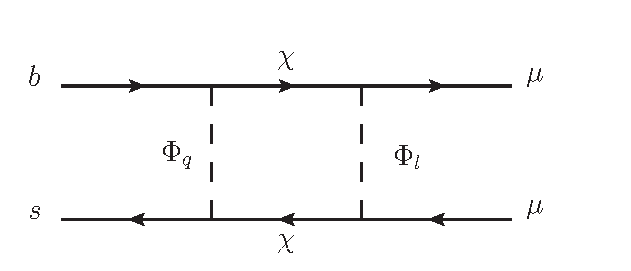
\includegraphics[width=0.6\textwidth]{../pics/bsmumu.eps}
 \caption{bs->mumu}
 \label{pic_Bsmumu}
\end{figure}
After we first focussed on a pure leptonic process, we add a quark pair. Our parameter set for this semileptonic process is now extended to
\begin{align}
 \left(m, M_l, M_q, g_2^l, g_2^q, g_3^q\right).
\end{align}
Box diagrams of the kind as in picture \ref{pic_Bsmumu} are usually not calculated 
all the way down to cross sections but one rather uses the formalism of effective field theory since the typical hadronic energy scale is of
$\mathcal{O}$(1 GeV) which is much lower than the weak scale $\mathcal{O}$(100 GeV) that is also the expected mass scale of our NP states. 
\\ \\ \noindent \textit{Matrix Element}\\
\noindent So we can use 
the OPE framework where they are integrated out and the external masses and momenta are set to zero. The amplitude in the full theory is
\begin{align}
 M =\alpha_i^{q*} \alpha_j^{q*} \alpha_m^l \alpha_n^l\int \frac{\dx^4 q}{(2\pi)^4} \frac{q^\rho}{q^2-m^2}\Delta_q \Delta_l \frac{q^\sigma}{q^2-m^2} \left(\bar L_L^n \gamma_\rho Q_L^j\right) \left(\bar Q_L^i \gamma_\sigma L_L^m\right)
 \label{eq_matElemBSmumu}
\end{align}
with $q$ as the internal momentum and the scalar propagators $\Delta = \frac{1}{q^2-M^2}$ and the $\ti\epsilon$ terms in the denominators are already omitted
due to Wick-rotation later on when the integral is performed. The reasons why $m$ in the fermion propagators is missing
and why there is a Lorentz structure in the couplings, are connected. Since we have a model which couples only to left handed particles $\psi_L = P_L \psi$,
the fermion currents look like $\bar \psi_L (\slashed{q}+m)\varphi_L = \bar \psi P_R (q^\mu \gamma_\mu+m) P_L\varphi$. Further
$\{P_{L,R},\gamma^\mu\} = \gamma^\mu P_{R,L}$, $P_{L,R}^2 = P_{L,R}$ and $P_R P_L = 0$, so we are left over with the four fermion expression in 
\eqref{eq_matElemBSmumu}. We can also reexpress $q^\rho q^\sigma = q^2 g^{\rho\sigma}/4$ under the integral. This results from spherical coordinates where
every combination $\rho\neq\sigma$ would include at least one uneven angular function. When the spherical integral is performed, they would lead to zero. The 
4 in the denominator is the spacetime dimension. The spherical integral $\dx \Omega$ itself just gives a $2\pi^2$ and we are left with the momentum integral
which is not problematic since it does not diverge
\begin{align}
 M \propto \frac{1}{32\pi^2} \int\limits_0^\infty \dx q \frac{q^5}{(q^2-m^2)^2(q^2-M_l^2)(q^2-M_q^2)} = \frac{K(x_q,x_l)}{64\pi^2 m^2}
\end{align}
with
\begin{align}
 K(x,y) &= \frac{K(x)-K(y)}{x-y} \stackrel{x\rightarrow y}{=} \frac13\\
 K(x)&=\frac{1-x+x^2\log(x)}{(x-1)^2} \stackrel{x\rightarrow 1}{=} \frac32.
\end{align}
In the SM, the fermion currents do not combine quarks and leptons. To compare the NP contribution to this process, we have to rearrange the fermion currents,
so that we have the same structure. This will be done by the Fierz identities.
\\ \\ \noindent \textit{Fierz Identities}\\
They usually relate a Dirac quadrilinear, containing four spinors, with a sum of rearranged Dirac quadrilinears \cite{Fierz}
\begin{align}
  \left[\bar w_1\Gamma_I^{} w_2\right] \left[\bar w_3 \Gamma^I w_4 \right] =: e_I(1234) = \sum\limits_J F_{IJ} e_J(1432)
\end{align}
with an (anti)spinor $w$ and $\Gamma_I$ as a set of Dirac matrices whereby $I=S,V,T,A,P$ representing $I,\gamma^\mu,\sigma^{\mu\nu},\gamma^\mu\gamma_5,\gamma_5$, 
respectively. The coefficients $F_{IJ}$ are real numbers and can differ for other arrangements.
% \begin{align}
%  F_{IJ}=\frac14\begin{pmatrix}
%     1&1&\frac12&-1&1\\
%     4&-2&0&-2&-4\\
%     12&0&-2&0&12\\
%     -4&-2&0&-2&4\\
%     1&-1&\frac12&1&1\\
%  \end{pmatrix}_{IJ}.
% \end{align}
\noindent For our purpose we want to transform the quadrilinear in \eqref{eq_matElemBSmumu}. By expanding there are four terms
\begin{align}
 e_V(1234)+e_A(1234)-\left(e'_V(1234) + e'_A(1234)\right).
 \label{eq_fierz}
\end{align}
The primed quadrilinears represent a pseudoscalar combination of two parity partners, e.g. $e'_V = \left[\bar w\gamma^\mu w\right]\left[w\gamma_\mu\gamma_5w\right]$
which are transformed with $F^\text{T}$. We can see that \eqref{eq_fierz} is an invariant for every order and so we can simply rearrange the quadrilinear.
\\ \noindent For later cases we also point out that 
\begin{align}
 \left[\bar w_1 P_R w_2\right]\left[\bar w_3 P_L w_4\right] = \frac12  \left[\bar w_1 \gamma_\mu P_L w_4\right]\left[\bar w_3 \gamma^\mu P_L w_2\right]
\end{align}

 \noindent \textit{Additional $SU(2)_L$-invariant term}\\
\noindent The operator $O_\delta=\left(\bar Q_L^i \gamma_\rho Q_L^j\right)\left(\bar L_L^m \gamma^\rho L_L^n\right)$ is not the only one which is a singlet
in the isospin space but $O_\tau=\left(\bar Q_L^i\vec \tau \gamma_\rho Q_L^j\right)\left(\bar L_L^m\vec \tau \gamma^\rho L_L^n\right)$ as well which enables
charged currents. The eventual operator is a superposition of these two. There might be several ways of computing the model dependent, relative 
prefactor $X$ of $O_\tau$  but one possibility is to regard the particles at each vertex as isospin multiplets. Since we want the vertices to be 
$SU(2)_L$-invariant, we 
decompose the product and focus on the singlet. This will be done for all four vertices per diagram which are multiplied and then added up for every diagram,
one can write down using these operators. For model A, this calculus can be done equivalently but can be skipped, because no charged currents as 
$b \bar u \rightarrow \mu \bar \nu$ are not induced, thus the prefactor of $O_\tau$ has to be zero and therefore 
\begin{align}
  \mathcal{L}^A_\text{eff} \supset \frac{K(x_q,x_l)}{m^2}\frac{\alpha_i^{q*} \alpha_j^{q*} \alpha_m^l \alpha_n^l}{64\pi^2} \times O_\delta.
 \label{eq_LagBSmumuModA}
\end{align}
In the case of higher dimensional isospin multiplets, processes of the just mentioned kind occur and thus we have three distinct types, with respect to 
their prefactor that can be checked by expanding $O_\delta + X O_\tau$, namely $\bar d d\rightarrow \bar l l$, $\bar d d \rightarrow \bar\nu \nu$ and 
$d \bar u\rightarrow l\bar\nu$. \\
\noindent To get the singlet expression we can make use of the Clebsch-Gordan coefficients, known from spin arithmetics which also obey an $SU(2)$-Group.
They can be read off the tables from (PDG). For a triplet ($\chi$) and two doublets ($\Phi$ and $D=Q,L$) we get
\begin{align}
 \frac{1}{\sqrt{3}}\left(\chi_3\Phi_1D_1 - \frac{1}{\sqrt{2}}\chi_2\left(\Phi_2D_1+\Phi_1 D_2\right) + \chi_1\Phi_2D_2 \right).
 \label{eq_CG}
\end{align}
The indices represent the components of the respective multiplets. One has to be careful which vertex one is looking at while using \eqref{eq_CG} in reference
to the Lagrangian \eqref{eq_modelLagrangian}. An incoming $u$-quark occupies the first isospin component in the quark doublet $Q$ but an outgoing one the 
second of $\bar Q$. Keeping this in mind we can look at each vertex of figure \ref{pic_Bsmumu} and examine the applicable coefficient. This is examplarily
depicted in figure \ref{pic_CG} for a generic $\bar d d\rightarrow \bar l l$ process that also represents $\bar b s \rightarrow \bar \mu \mu$.
\begin{figure}[t]
 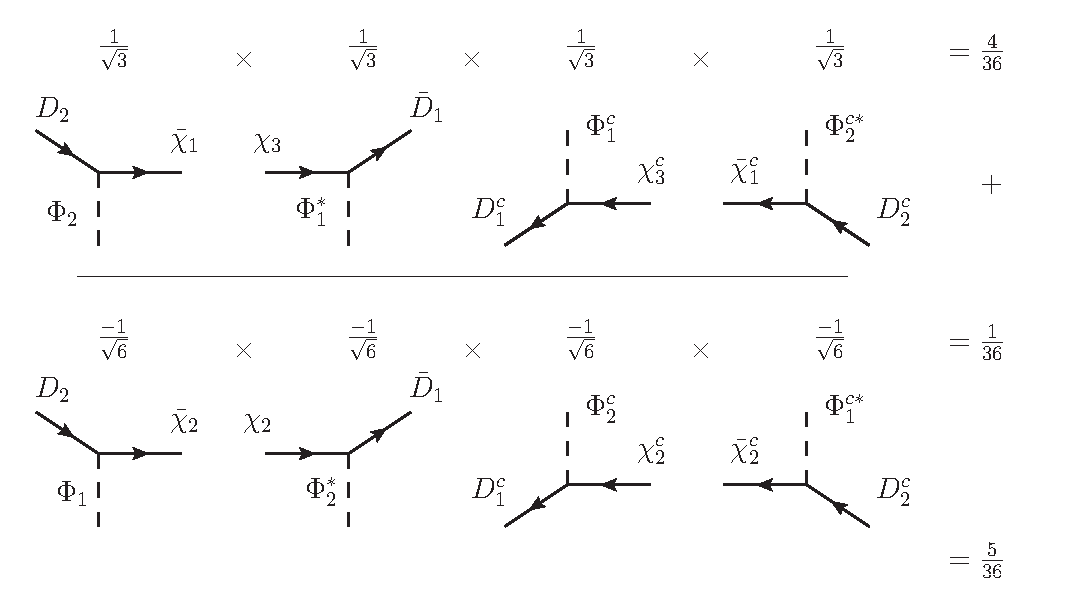
\includegraphics[width=\textwidth]{../pics/CG.eps}
 \caption{$SU(2)_L$ singlet representation at each vertex of figure \ref{pic_Bsmumu} with the respective Clebsch-Gordan coefficients from \eqref{eq_CG}. 
 This is exemplary for $\bar d d\rightarrow \bar d d$ processes which get contributions from two different particle configurations.}
 \label{pic_CG}
\end{figure}
This gives an overall factor of $\sfrac{5}{36}$. The computation for the remaining two types is similar and yields $\sfrac{4}{36}$ for 
$\bar d d\rightarrow \bar \bar \nu \nu$ and $\sfrac{1}{36}$ for $\bar u d \rightarrow \bar \nu l$. With these three fractions and the relations from $O_\delta + X O_\tau$
we can extract the prefactor $X=\sfrac23$. Finally, we can write down the effective Lagrangian for the triplet case
\begin{align}
 \mathcal{L}^B_\text{eff} \supset \frac{K(x_q,x_l)}{m^2}\frac{\alpha_i^{q*} \alpha_j^{q*} \alpha_m^l \alpha_n^l}{64\pi^2}\times\left(O_\delta + \frac23 O_\tau\right).
 \label{eq_LagBSmumuModB}
\end{align}
\\ \textit{Crossed Boxes}\\
\noindent As we assume our DM candidate $\chi^0$ to be Majorana, there are also contributions from crossed boxes (fig. \ref{pic_crossed}) for uncharged
currents like our process of interest $\bar d d\rightarrow \bar l l$. Compared to the former matrix element \eqref{eq_matElemBSmumu} we have some changes
for the crossed box diagram. Using the Feynman rules for internal Majorana particles and the commutation rules for $C$ from section \ref{sec_Majorana}, 
we see that now the masses in the fermion propagators remain. The fierzing of the four fermions gives a $\sfrac12$ since we do not have initial $\gamma$s
between them. The momentum integral similarly to the pure Dirac case yields
\begin{align}
 M_\text{box} \propto \frac{1}{64 \pi^2}\int\limits_0^\infty \dx q \frac{q^3 \cdot m^2}{(q^2-m^2)^2(q^2-M_l^2)(q^2-M_q^2)} = \frac{G(x_q,x_l)}{128\pi^2m^2}
\end{align}
with similar loop functions
\begin{align}
 G(x,y) &= \frac{G(x)-G(y)}{x-y}\stackrel{x\rightarrow y}{=} -\frac16\\
 G(x)&=\frac{1-x+x\log(x)}{(x-1)^2} \stackrel{x\rightarrow 1}{=} \frac12.
\end{align}
Concerning the $SU(2)_L$ invariance, the crossed box can just have the uncharged particle state for the internal lines. Therefore one gets only $\sfrac{1}{36}$
which is one fifth of the bare Dirac contribution. The two terms with $K(x_q,x_l)$ and $G(x_q,x_l)$, respectively, have opposite signs so that they can cancel
each other out and hence may reduce the impact of constraints from observables.\\
\\ \textit{New Physics Contribution}\\
\noindent Now we will gather up the information to get another bound for our model. There are two operators in the effective Hamiltonian for $B_s\rightarrow \mu\mu$
transitions, $O_9$ and $O_{10}$ (sec. \ref{sec_EFT}). The expression for the Wilson coefficient $C_9 = -C_{10}$ (1408.1627) is obtained by comparing the coefficients from the 
4-fermi operator in the effective Lagrangians and the effective Hamiltonian
\begin{align}
 C_9^A &= N \frac{g_s^*g_b|g_\mu|^2}{m^2} \frac{1}{128\pi^2} \left(K(x_q,x_l) + G(x_q,x_l)\right)\\
 C_9^B &= N \frac{g_s^*g_b|g_\mu|^2}{m^2} \frac{5}{384\pi^2} \left(K(x_q,x_l) + \frac15 G(x_q,x_l)\right)
\end{align}
with
\begin{align}
 N = \left(\frac{4G_F}{\sqrt{2}} V_{ts}^*V_{tb} \frac{\alpha_\text{EM}}{4\pi}\right)^{-1}.
\end{align}

% Prefactors for other representations are listed in table below.

% \begin{table}[h]
% \begin{tabular}{c|cccc}
%  $(\chi,\Phi)$& (1,2) & (3,2) & (4,3) & (5,4)\\
%  \hline
%  $X$ & $0$ & $\sfrac23$ & $\sfrac59$ & $\sfrac12$
%  \end{tabular}
%  
% \end{table}


\subsection{$B_s$-Mixing}
\begin{figure}[t]
 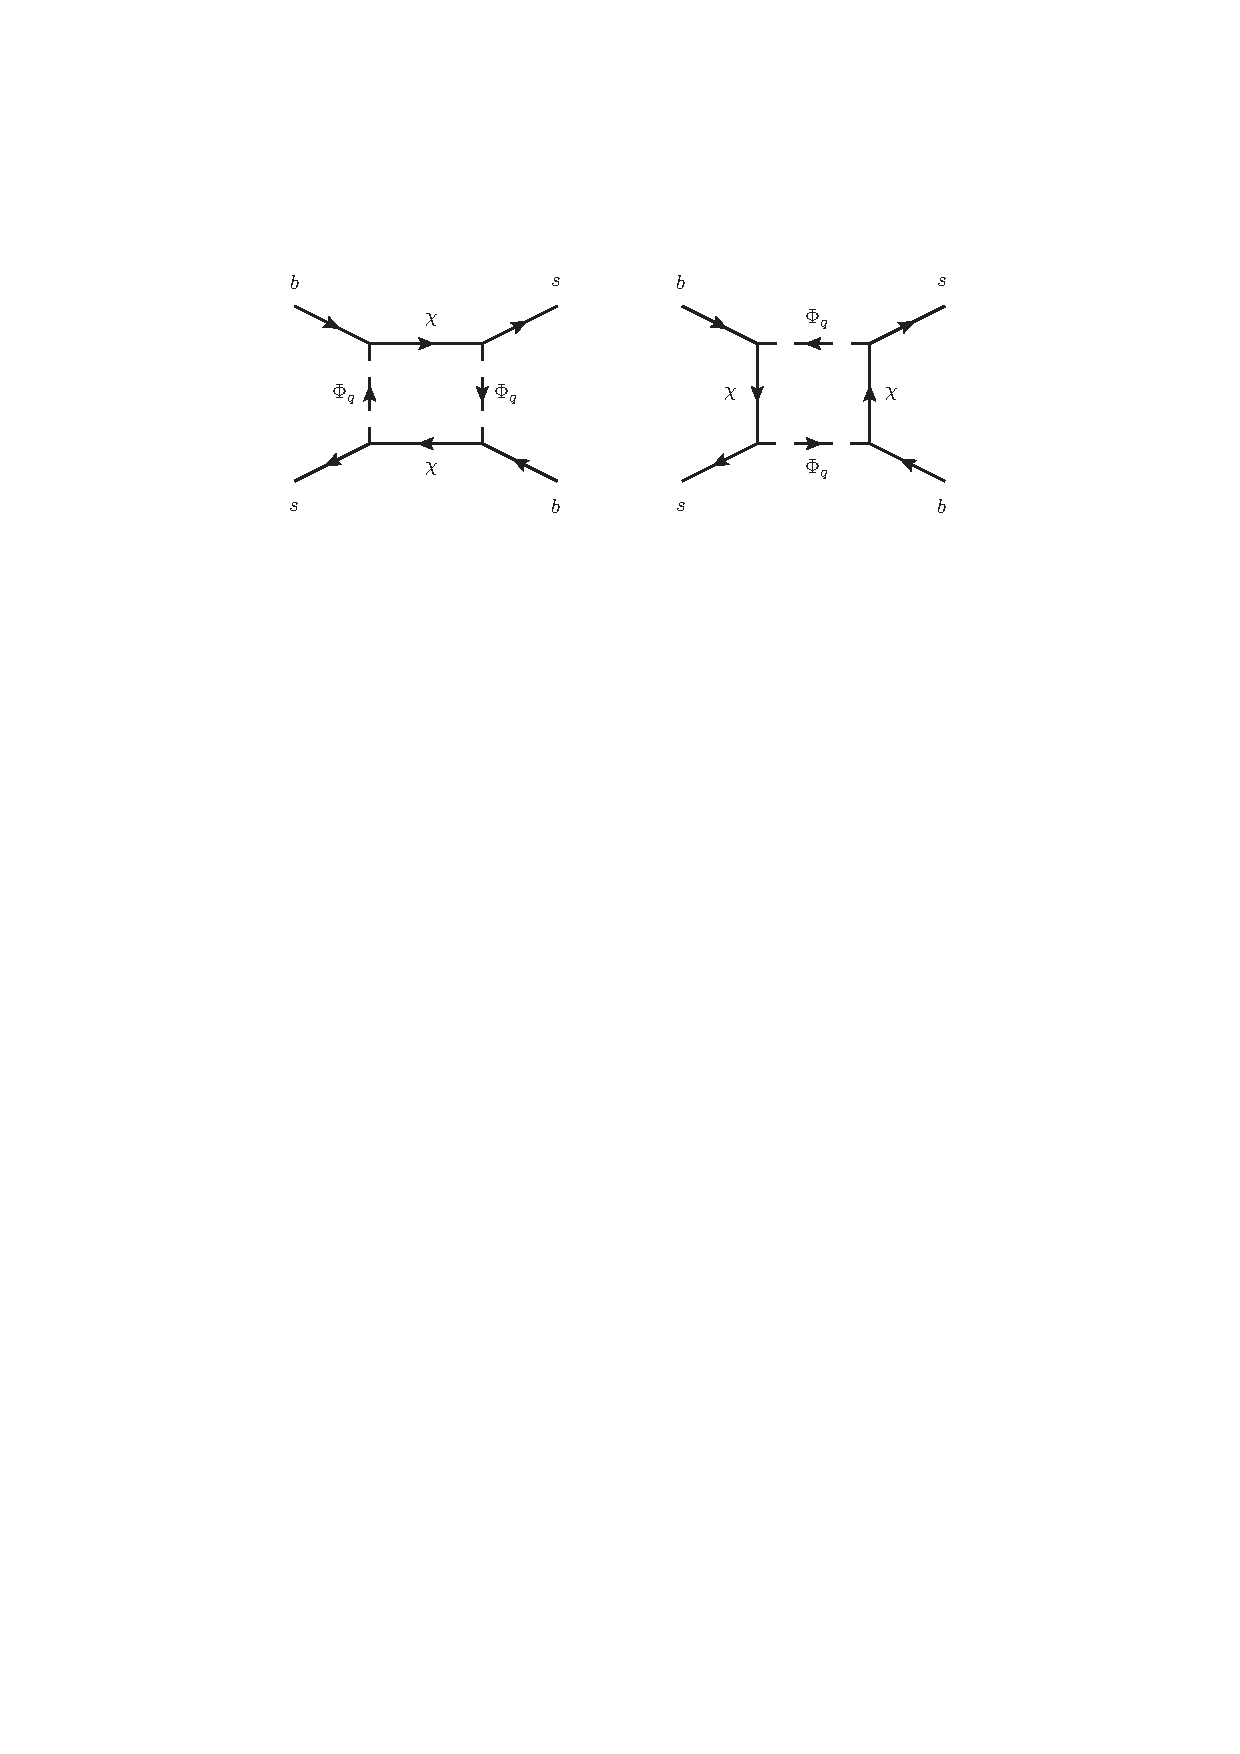
\includegraphics[width=0.6\textwidth]{../pics/bsmix.pdf}
 \caption{$B_s$-mixing. The crossed boxes also occur, see fig. \ref{pic_Bsmumu}}
 \label{pic_Bsmix}
\end{figure}
When there are semileptonic meson decays, hadronic ones are accordingly enabled.The diagrams for $B_s$-mixing are depicted in figure \ref{pic_Bsmix}. 
The parameter set only consists of
\begin{align}
 \left(m_\chi,M_q\right)
\end{align}
Other
meson mixings like $K\bar K$ or $ D \bar D$ are suppressed due to their smaller Yukawa couplings. From a calculational point of view, this process is 
quite similar to the former $b\rightarrow s\bar\mu\mu$ and is induced only through one-loop box diagrams in the SM to lowest order. The effective Hamiltonian
involves only one operator $(\bar s \gamma^\mu P_L b)(\bar s \gamma_\mu P_L b)$ for our chiral theory whose Wilson coefficient reads
\begin{align}
 C_{B\bar B}^A &=  \frac{|g_2^{q*}g_3^q|^2}{m^2} \frac{1}{128\pi^2} \left(K'(x_q) + G'(x_q)\right)\\
 C_{B\bar B}^B &=  \frac{|g_2^{q*}g_3^q|^2}{m^2} \frac{5}{384\pi^2} \left(K'(x_q) + \frac15 G'(x_q)\right)
 \label{eq_WilsonMix}
\end{align}
with the first derivatives $K'(x)$ and $G'(x)$ being the limits of $K(x,y)$ and $G(x,y)$, respectively, for $y\rightarrow x$. 



\subsection{Anomalous Magnetic Moment of the Muon}
The NP contributions for the anomalous magnetic moment of the muon are discribed by the parameter set 
\begin{align}
 \left\{m, M_l, g_2^l\right\}.
\end{align}
The Feynman diagram for this process is depicted in figure \ref{pic_g-2}. 
\begin{figure}[t]
 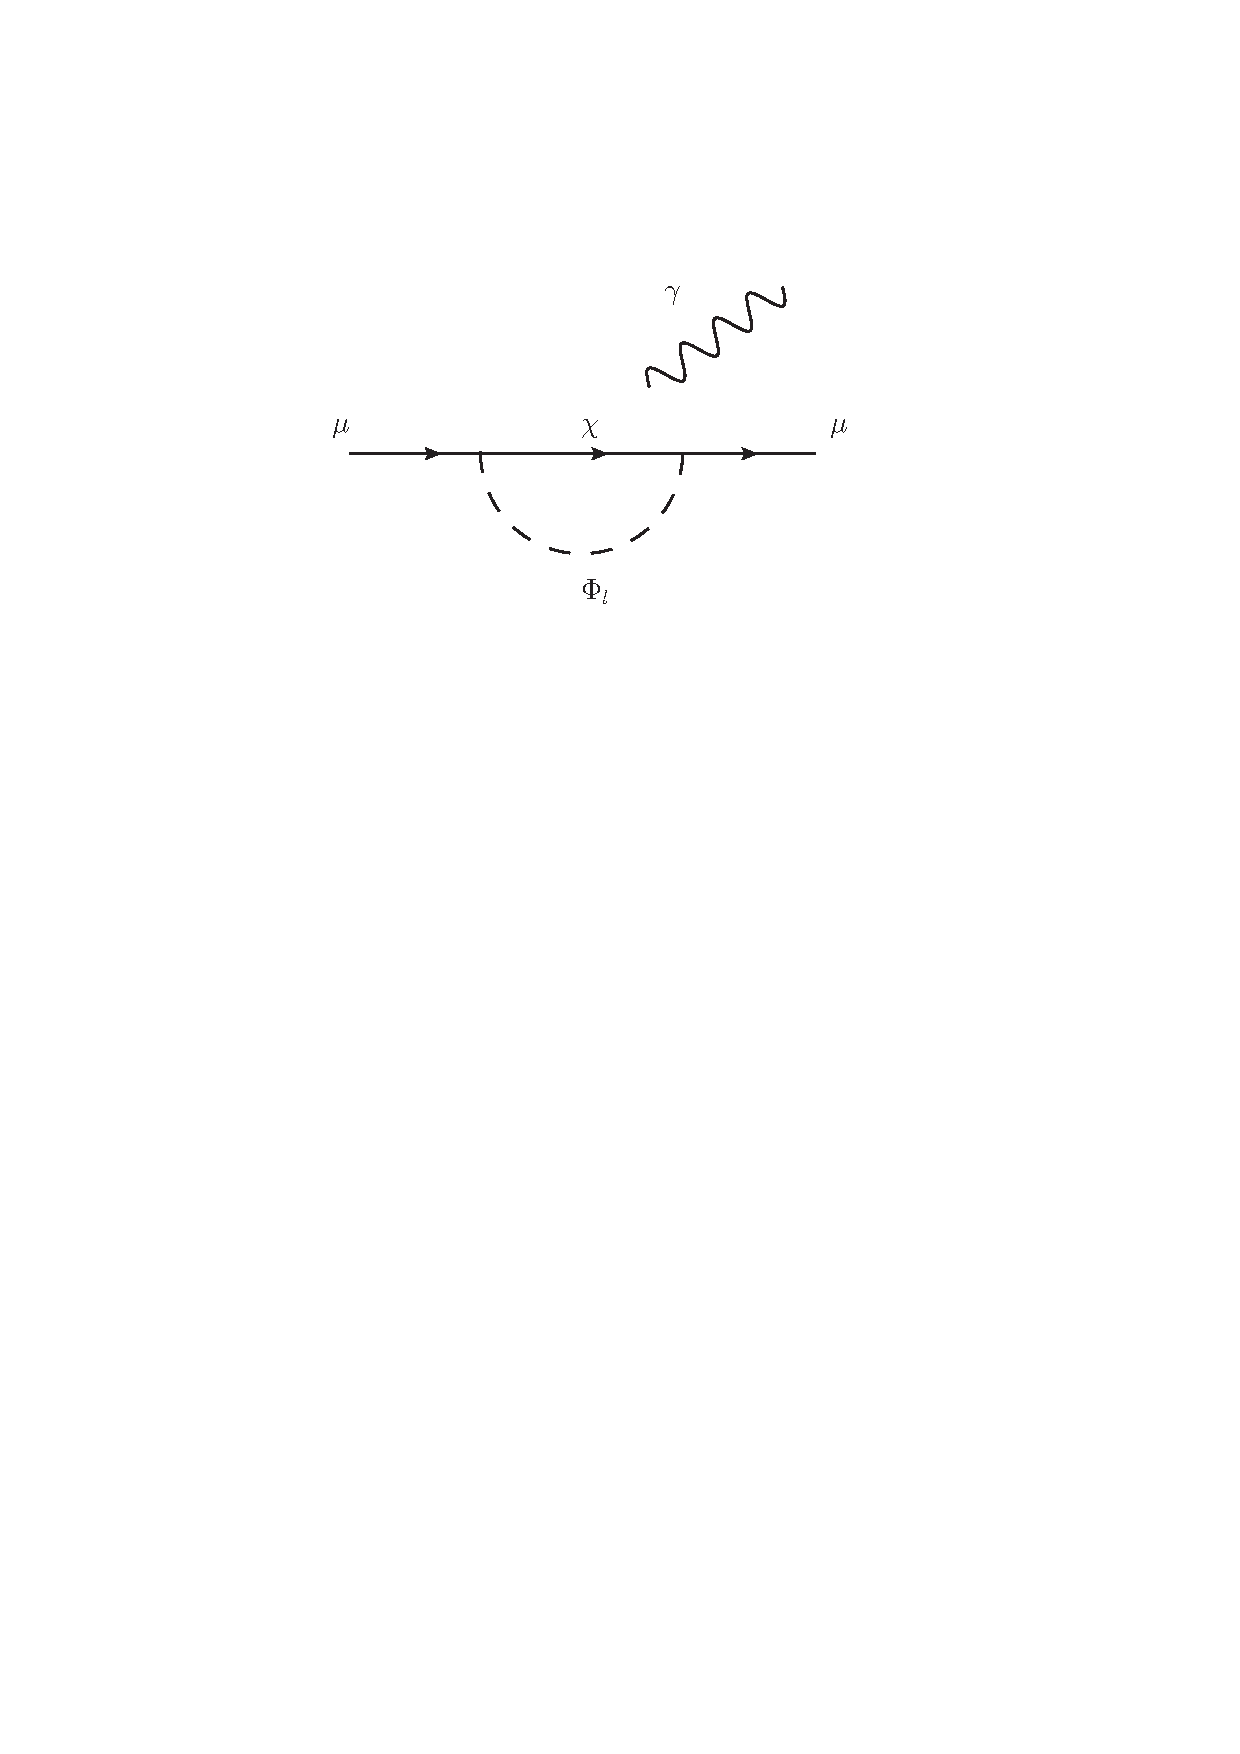
\includegraphics[width=0.6\textwidth]{../pics/g-2.pdf}
 \caption{One-loop contribution to $a_\mu$. Depending on the representations, there are multiple possibilites to attach the photon.}
 \label{pic_g-2}
\end{figure}
Depending on which particle in the loop the photon interacts, there is a different matrix element. If it couples to the scalar, it reads as
\begin{align}
 \mathcal{M}^\rho = |g_2^l|^2 Q_{\Phi_l} e \int\frac{\dx^4 k}{(2\pi)^4} \left[ \frac{2k_\mu k^\rho}{D^\chi_kD^l_{k-p_1}D^l_{k-p_2}} - \frac{k_\mu\left(p_1 +p_2\right)^\rho}{D^\chi_kD^l_{k-p_1}D^l_{k-p_2}} \right]\times \bar\mu_L(p_2)\gamma^\mu\mu_L(p_1) 
 \label{eq_matg2}
\end{align}
where $Q_{\Phi_l}$ is the electric charge of the boson, $\ti e(2k-p_1-p_2)^\mu$ is the scalar-photon coupling \cite{MDSchwartz}. 
The free Lorentz-index gets contracted with
the polarisation vector $\epsilon_\rho$ of the external photon. With the Gordon idendity the vectorial operator is replaced by 
$\sigma^{\mu\nu}q_\nu/2m$ which is necessary to proceed (see sec. \ref{sec_flAnom}). The momentum integral (see \eqref{eq_g2loops})
can be performed \cite{Lavoura} 
where we neglect the external mass and use $q^2=(p_1^2-p_2^2) = 0$ for an on-shell photon. The divergent term from the first term in \eqref{eq_matg2}
cancels out with two-point functions. 
Note that the notation in \cite{Lavoura} is slightly different from ours due to the relative inversion of the squared mass 
fraction $x_l$. 
After gathering everything up and performing the calculation for the fermionic case, we have
\begin{align}
 M^\rho = \frac{|g^l_2|^2}{16\pi^2} \frac{m^2_\mu}{m_\chi^2}\left(Q_\chi^i I(x_l) + Q_{\Phi_l}^i \frac{1}{x_l} I(x_l^{-1}) \right)\times \bar \mu_L\frac{e\ti\sigma^{\rho\nu}q_\nu}{2m_\mu} \mu_L,
 \label{eq_g-2}
\end{align}
where the sum over $i$ is understood so that for the electric charges, $Q_\mu = Q_\chi - Q_{\Phi_l}$ is ensured and $I$ is a loop function 
(see \eqref{eq_loopmuon}). The NP contribution to $\Delta a_\mu$ can be read off \eqref{eq_g-2}.



% \begin{align}
%  \left(m, M_q, g_3^{q*}g_2^q\right).
% \end{align}
% \begin{align}
%  \mathcal{L}_\text{eff} \supset \frac{K'(x_q)}{m^2}\frac{\alpha_i^{q*} \alpha_j^{q*} \alpha_m^l \alpha_n^l}{128\pi^2}\times\left(O_\delta + \frac23 O_\tau\right).
%  \label{eq_LagBSmixModB}
% \end{align}

\subsection{Direct Detection}
\label{sec_ddphen}
In this section the phenomenological aspects of DM itself are focussed.
We start with direct detection (DD) or nucleon ($N$) scattering where a DM particle scatters off a parton (quark or gluon) of a nucleon. 
\\ \\ \textit{Effective Lagrangian}\\
The process arises
due to a spin independent (SI) or spin dependent (SD) interaction \eqref{eq_th.sigma.dd} which are described by an effective Lagrangian \cite{1104.0228}
\begin{align}
 \mathcal{L}^\text{eff} = \sum\limits_{q,Q} \mathcal{L}^\text{eff}_{q,Q} + \mathcal{L}^\text{eff}_g.
\end{align}
We use $q$ for the light quarks $u$, $d$, $s$ and $Q$ for heavier $c$, $b$, $t$ and $g$ for gluons. \eqref{eq_fierzSPtoVA} shows that this chiral model
only provides effective interactions with quarks as $\bar \chi\gamma^\mu\chi \bar q\gamma_\mu q$ and $\bar \chi\gamma^\mu\gamma_5 \bar q\gamma_\mu \gamma_5 q$
as six dimensional operators. The former vanishes for Majorana DM. The latter is SD 
and the resulting cross section can be evaluated with the expressions given in \cite{1104.0228} for the leading processes to be of
order $\mathcal{O}(10^{-44})$ cm$^2$. But the upper limits obtained by IceCube \cite{1212.4097} yield $\mathcal{O}(10^{-40})$ cm$^2$ for 
a 100 GeV DM particle.
Therefore we can neglect them. A possibly occuring scalar operator $f_q m_q\bar \chi \chi \bar q q$ also vanishes for tree level processes in our chiral model
but is enabled at loop level. Therefore the first contributing
SI operators coming from quark interactions are eight dimensional, namely those depending on twist-2 operators. They are the traceless parts of the
quark energy momentum tensor and arise from the matrix element of a quark current product expressed in local operators \cite{MDSchwartz}. 
% The twist of an operator is definded as the difference between its mass dimension and its spin. 
\\ \noindent Since our DM particle shall be an 
$SU(3)_C$-singlet, it does not couple directly to gluons $g$ but scalarlike at one-loop level through the heavy quarks. There is also a twist-2 
operator for the gluon but its coefficient will be suppressed by $\alpha_s$ so we will not consider it further. For the $SU(2)_L$ singlet
DM particle, which does not interact with the $W$ bosons, the leading SI Lagrangian is
%For both DM $SU(2)_L$-representations, the singlet and the triplet, the leading SI operators are
\begin{align}
 \mathcal{L}^\text{eff} =&\, \frac{g_q^{(1)}}{m_\chi} \bar \chi\ti \partial_\mu \gamma_\nu\chi O_q^{\mu\nu} + \frac{g_q^{(2)}}{m^2_\chi} \bar \chi(\ti \partial_\mu) (\ti\partial_\nu)\chi O_q^{\mu\nu} \\
 \nonumber
 &+ f_G \bar \chi \chi G^a_{\mu\nu} G^{a\mu\nu}.
\end{align}
The twist-2 operator for the quark is
\begin{align}
 O_q^{\mu\nu} = \frac12 \bar q \ti \left(D^\mu \gamma^\nu + D^\nu \gamma^\mu - \frac12 g^{\mu\nu} \slashed{D}\right) q
\end{align}
with $D_\mu$ as the covariant derivative for $SU(3)_C$. The three coefficients of mass dimension $-3$ ($g_q^{(1)}$, $g_q^{(2)}$, $f_G$) enter 
the form factor $f_N$ in \eqref{eq_th.sigma.dd} as
\begin{align}
 \frac{f_N}{m_N} = \sum\limits_{q,c,b} \frac34 \left(q(2)+\bar q(2)\right) \left(g_q^{(1)} + g_q^{(2)}\right) - \frac{8\pi}{9\alpha_s}f_{TG}f_G
 \label{eq_ddformfactorA}
\end{align}
where the matrix elements of the effective operators are expressed with the nucleon mass $m_N$ as \cite{1007.2601}
\begin{subequations}
\begin{align}
 \langle N(p)| O_q^{\mu\nu} | N(p)\rangle =& \frac{1}{m_N}\left(p^\mu p^\nu - \frac14 m_N^2 g^{\mu\nu}\right) \left(q(2) + \bar q(2)\right),\\
 f_{TG} :=& 1- \sum\limits_q f_{Tq},\\
 f_{Tq} :=& \langle N|m_n \bar qq |N\rangle /m_N.
\end{align}
\end{subequations}
The quantities $q(2)$ and $\bar q(2)$ are the second moments \cite{0811.1779} of the parton distribution function (PDF) of quark $q(x)$ or antiquark 
$\bar q(x)$, respectively, in the nucleon $q(2)+\bar q(2) = \int_0^1 \dx x\, x^2 \left[q(x) + \bar q(x)\right]$. The values used for the numerical
calculation are listed in table \ref{tab_parton}.
\begin{table}[b]
 \begin{tabular}{c|ccccc}
   & $u$ & $d$ & $s$ & $c$ &$b$ \\
   \hline
  $q(2)$ & 0.22 & 0.11 & 0.026 & 0.019 & 0.012\\
  $\bar q(2)$ & 0.034 & 0.036 & 0.026 & 0.019 & 0.012\\
  $f_{Tq}$ & 0.020& 0.026 &\hspace{0.47cm}  0.134\cite{1209.3641}\\
 \end{tabular}
\caption{Second moments $q(2)$, $\bar q(2)$ of the quark PDFs evaluated at $\mu=m_Z$ and taken from \cite{0201195} and scalar matrix elements $f_{Tq}$ of 
the light quarks for the 
proton each. For the neutron $u(2)$ and $d(2)$ just swap and $f_{Tu}$ and $f_{Td}$ differ slightly \cite{9506380}. All other quantities are the same. }
\label{tab_parton}
\end{table}
\noindent The evaluation of $f_G$ is factorised in a short distance and a long distance 
contribution. The former (latter) represents a scale of heavy (light) particles as the colored scalar mediator (quarks). 
While the full loop process has to be calculated for the short distance (see fig. \ref{pic_ddsinglet}c), the long distance term can be thought of
as a triangle diagram (see fig. \ref{pic_ddsinglet}b) where $\Phi_q$ integrated 
out i.e. there arises a four fermion operator $f_Q m_Q \bar \chi \chi\bar Q Q$. The long distance gluonic form factor is expressed by $f_Q$ 
which are multiplied by a constant 
$c_Q = 1+11\alpha_s(m_Q)/4\pi$, ($c_c=1.32$, $c_b = 1.19$, $c_t = 1$)
resulting from large QCD corrections \cite{Djouadi}.
Due to their masses being smaller than $\Lambda_\text{QCD} = \mathcal{O}$(100 MeV), light quarks $q$ have a vanishing contribution to the long
distance term. Thus, we do not have to take them into account. The operator coefficients \eqref{eq_ddformfactorA} are determined for the 
singlet case.
\\ \\ \textit{Singlet Dark Matter}\\
\begin{figure}[t]
 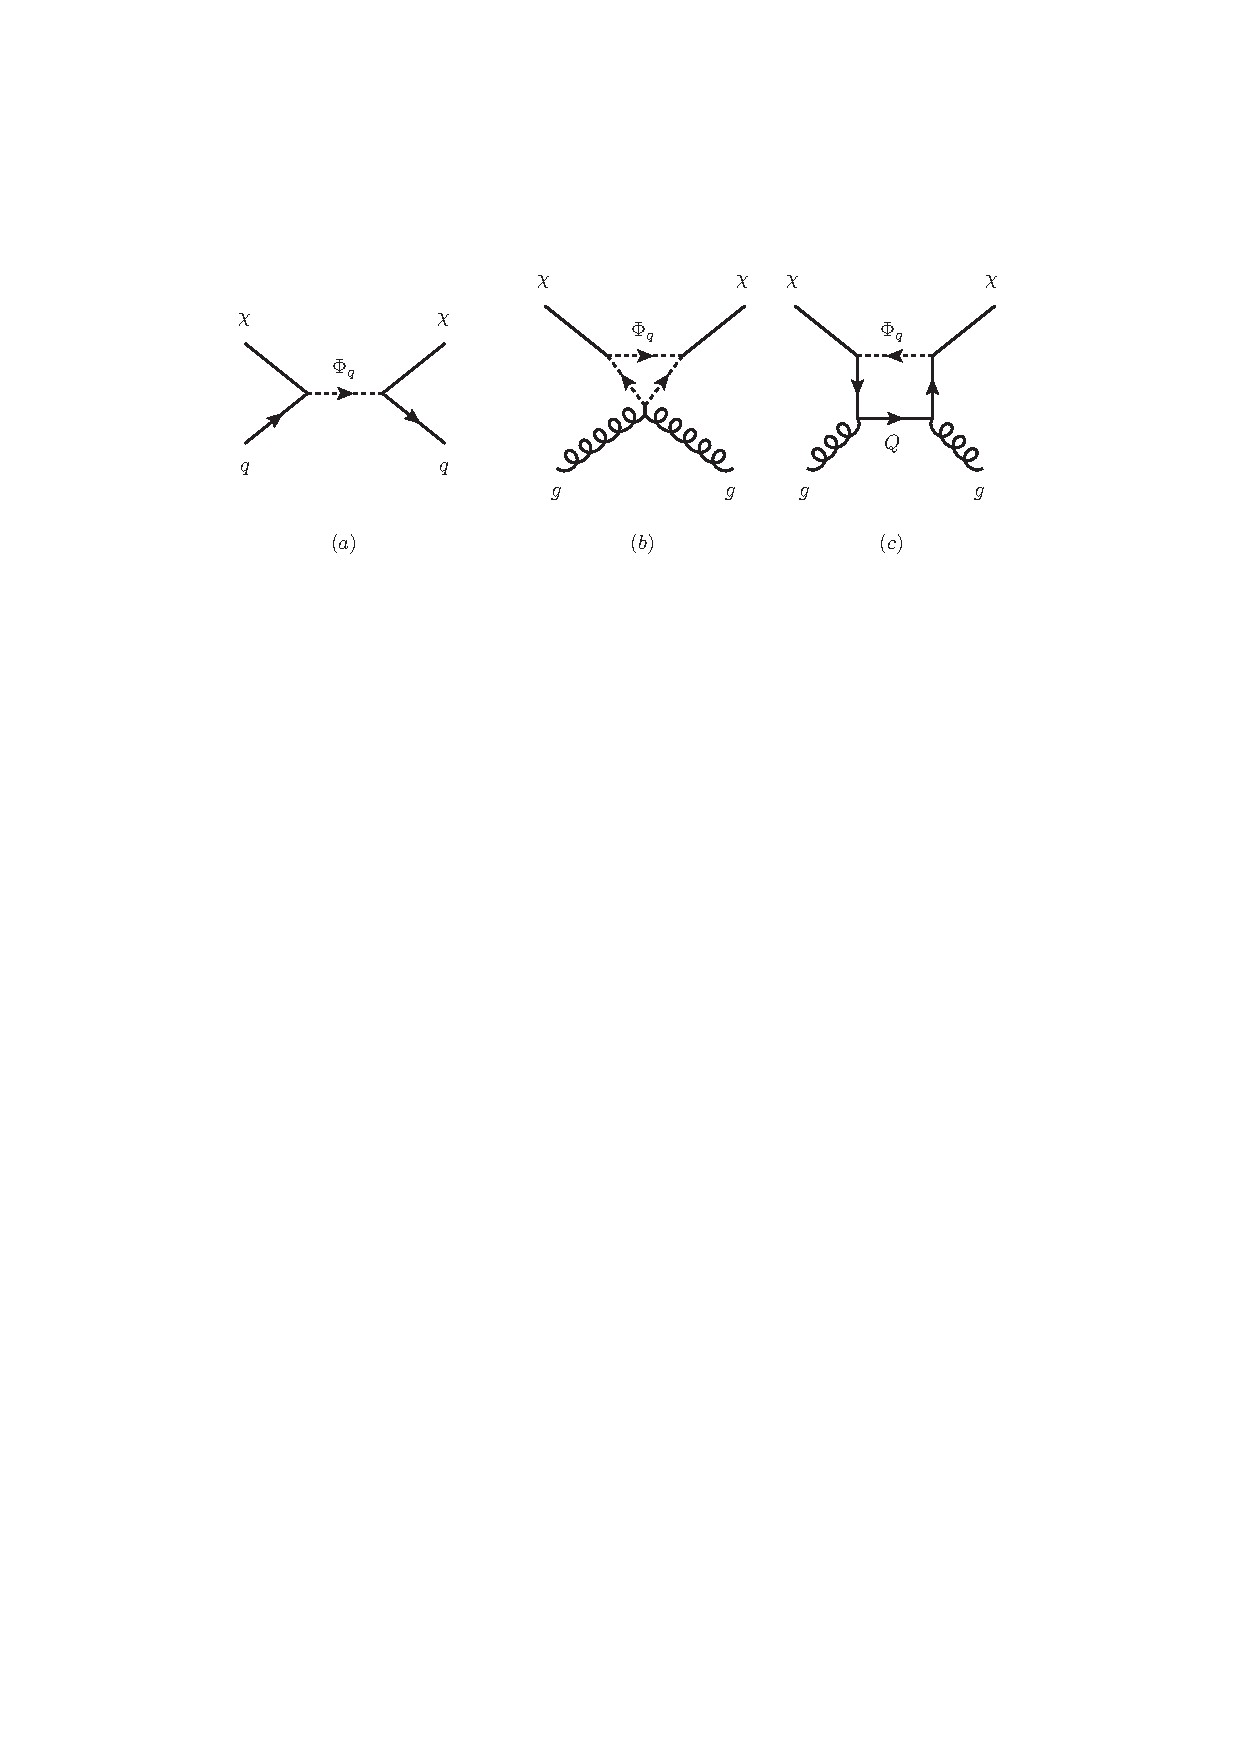
\includegraphics[width=1\textwidth]{../pics/ddsinglet.pdf}
 \caption{DM scatters off quarks at tree level and off gluons at one loop order.}
 \label{pic_ddsinglet}
\end{figure}
\noindent The $\chi$-$q$ interaction is visualised in figure \ref{pic_ddsinglet}a and is expressed by this s-channel process. After integrating out 
the scalar and in the massless quark limit the coefficients are
\begin{align}
 g_q^{(1)} = \frac{|g_q|^2 }{4} \frac{m_\chi}{\left(m_\chi^2 - M_{\Phi_q}^2\right)^2},\hspace{3cm} g_q^{(2)} = 0.
\end{align}
We assume the scalar to be much heavier than the fermion which is why possible divergencies due to mass degeneracy of DM and messenger have not
to be considered. 
The effective gluonic coupling in the 
singlet case is derived from the loop processes (see fig. \ref{pic_ddsinglet}b, c) 
% \begin{figure}[t]
%  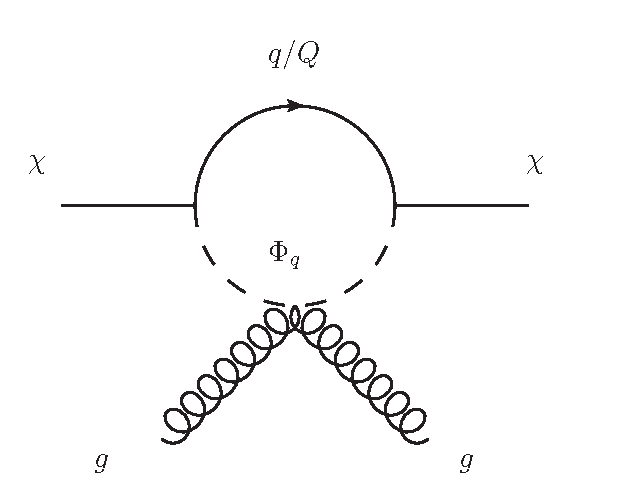
\includegraphics[width=0.5\textwidth]{../pics/phigluon.eps}
%  \caption{One loop diagrams contributing to the effective gluonic coupling.}
%  \label{pic_ddGluonA}
% \end{figure}
where we use the Fock-Schwinger gauge for the gluon
field $x^\mu G^a_\mu = 0$. The short distance (S) and long distance (L) terms are
\begin{align}
 f_G^\text{S}|_q = \frac{\alpha_s}{32\pi} m_\chi f^s,\hspace{3cm} f_G^\text{L}|_q = \frac{\alpha_s}{32\pi} m_\chi f^l
 \label{eq_ldsdLoop}
\end{align}
The loop functions $f$ (see \eqref{eq_singletloop}) are used at zero quark mass and the scalar mass being much larger than the DM mass.
In total, the scalar $\chi$-$g$ interaction coefficient reads
\begin{align}
 f_G = -\frac{\alpha_s}{96\pi} \frac{m_\chi}{M_{\Phi_q}^4} \sum\limits_{\text{all}} |g^q|^2
\end{align}
and the full form factor \eqref{eq_ddformfactorA} can be written in these limits as
\begin{align}
 \frac{f_N}{m_N} = \frac{m_\chi}{M_{\Phi_q}^4} \sum\limits_{q,Q} \left|g^q\right|^2 \left[\frac{f_{TG}}{108} + \frac{3}{12}\left(q(2) + \bar q(2)\right)\right].
 \label{eq_siformsinglet}
\end{align}
With their high Yukawa couplings, the bottom and top quark dominate the form factor. Inserting \eqref{eq_siformsinglet} into \eqref{eq_th.sigma.dd}
yields for a 100 GeV DM fermion and a 1 TeV messenger, the SI $\chi$-$N$ cross section computes to $\mathcal{O}(10^{-49}$ cm$^2$). This is far below
current bounds. Hence, testing the singlet case by direct detection is currently impossible.
\\ \\ \textit{Triplet Dark Matter}\\
\begin{figure}[t]
 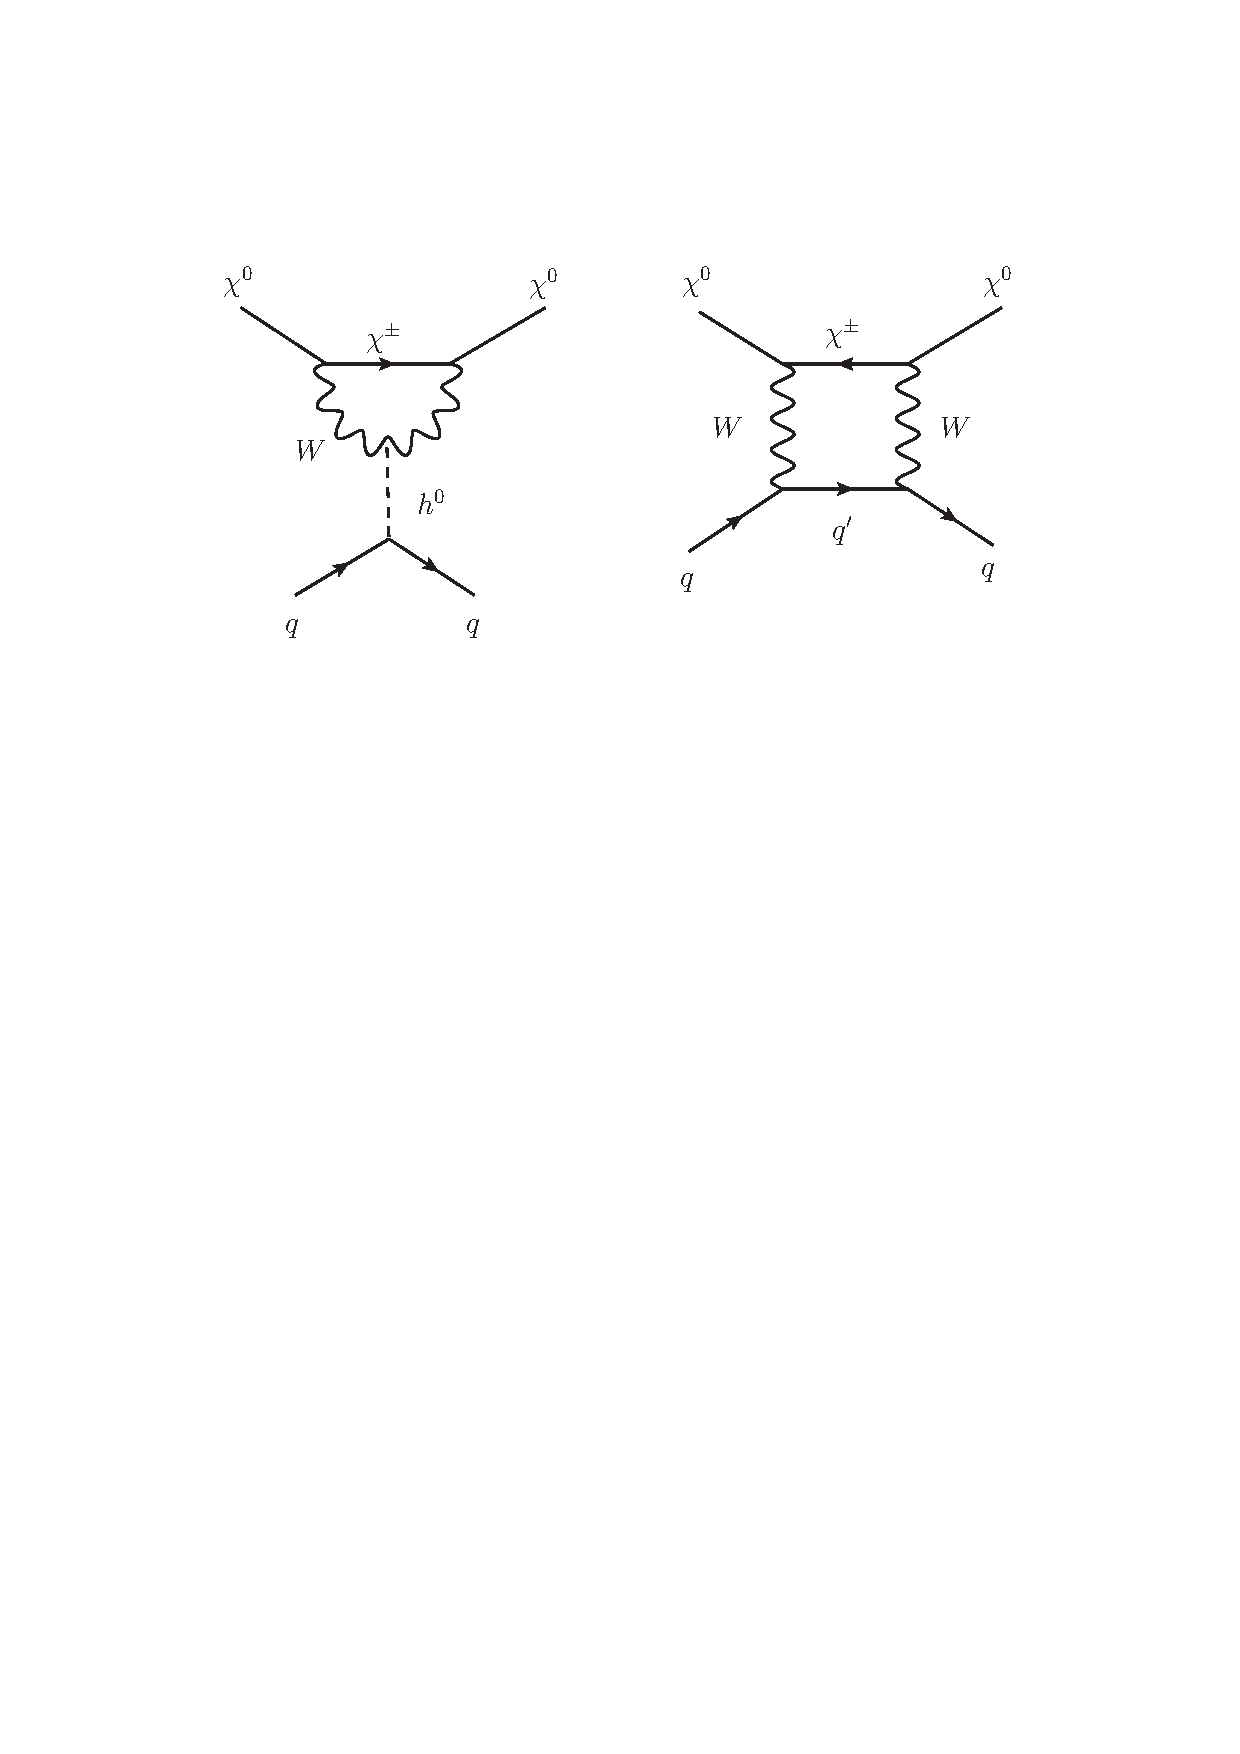
\includegraphics[width=0.7\textwidth]{../pics/wloops.pdf}
 \caption{One loop processes for the effective $\chi^0-N$ coupling. Penguins with a photon or a $Z$-boson turn out to vanish(\cite{1104.0228}).}
 \label{pic_wloop}
\end{figure}
\noindent The main difference between the $SU(2)_L$ singlet and the triplet is the interaction with the weak boson $W$. While the singlet does not couple to
it directly, the $W$ couples to two particle states within the triplet whose electric charges differ by one. To remind, in neither case the 
DM particle carries hypercharge, so that the respective neutral component does not couple to the $Z$ boson. The interaction Lagrangian with the $W$ 
boson is 
\begin{align}
 \mathcal{L} = \frac{g_2}{\sqrt{2}} \left[\bar \chi^0 \gamma^\mu \chi^- W^+_\mu + \bar \chi^0 \gamma^\mu \chi^+W^-_\mu\right] +\, \text{h.c.}
\end{align}
Since the cross section in the singlet case was suppressed by the large scalar mass we can take advantage of the possible 
processes for direct detection which do not involve the scalar \cite{1004.4090}. In fact, the form factor is dominated by one loop processes with a 
$W$ for an interaction with quarks (see fig. \ref{pic_wloop}) and two loop processes for gluonic scattering (see fig. \ref{pic_2loopgluon}).
\begin{figure}[t]
 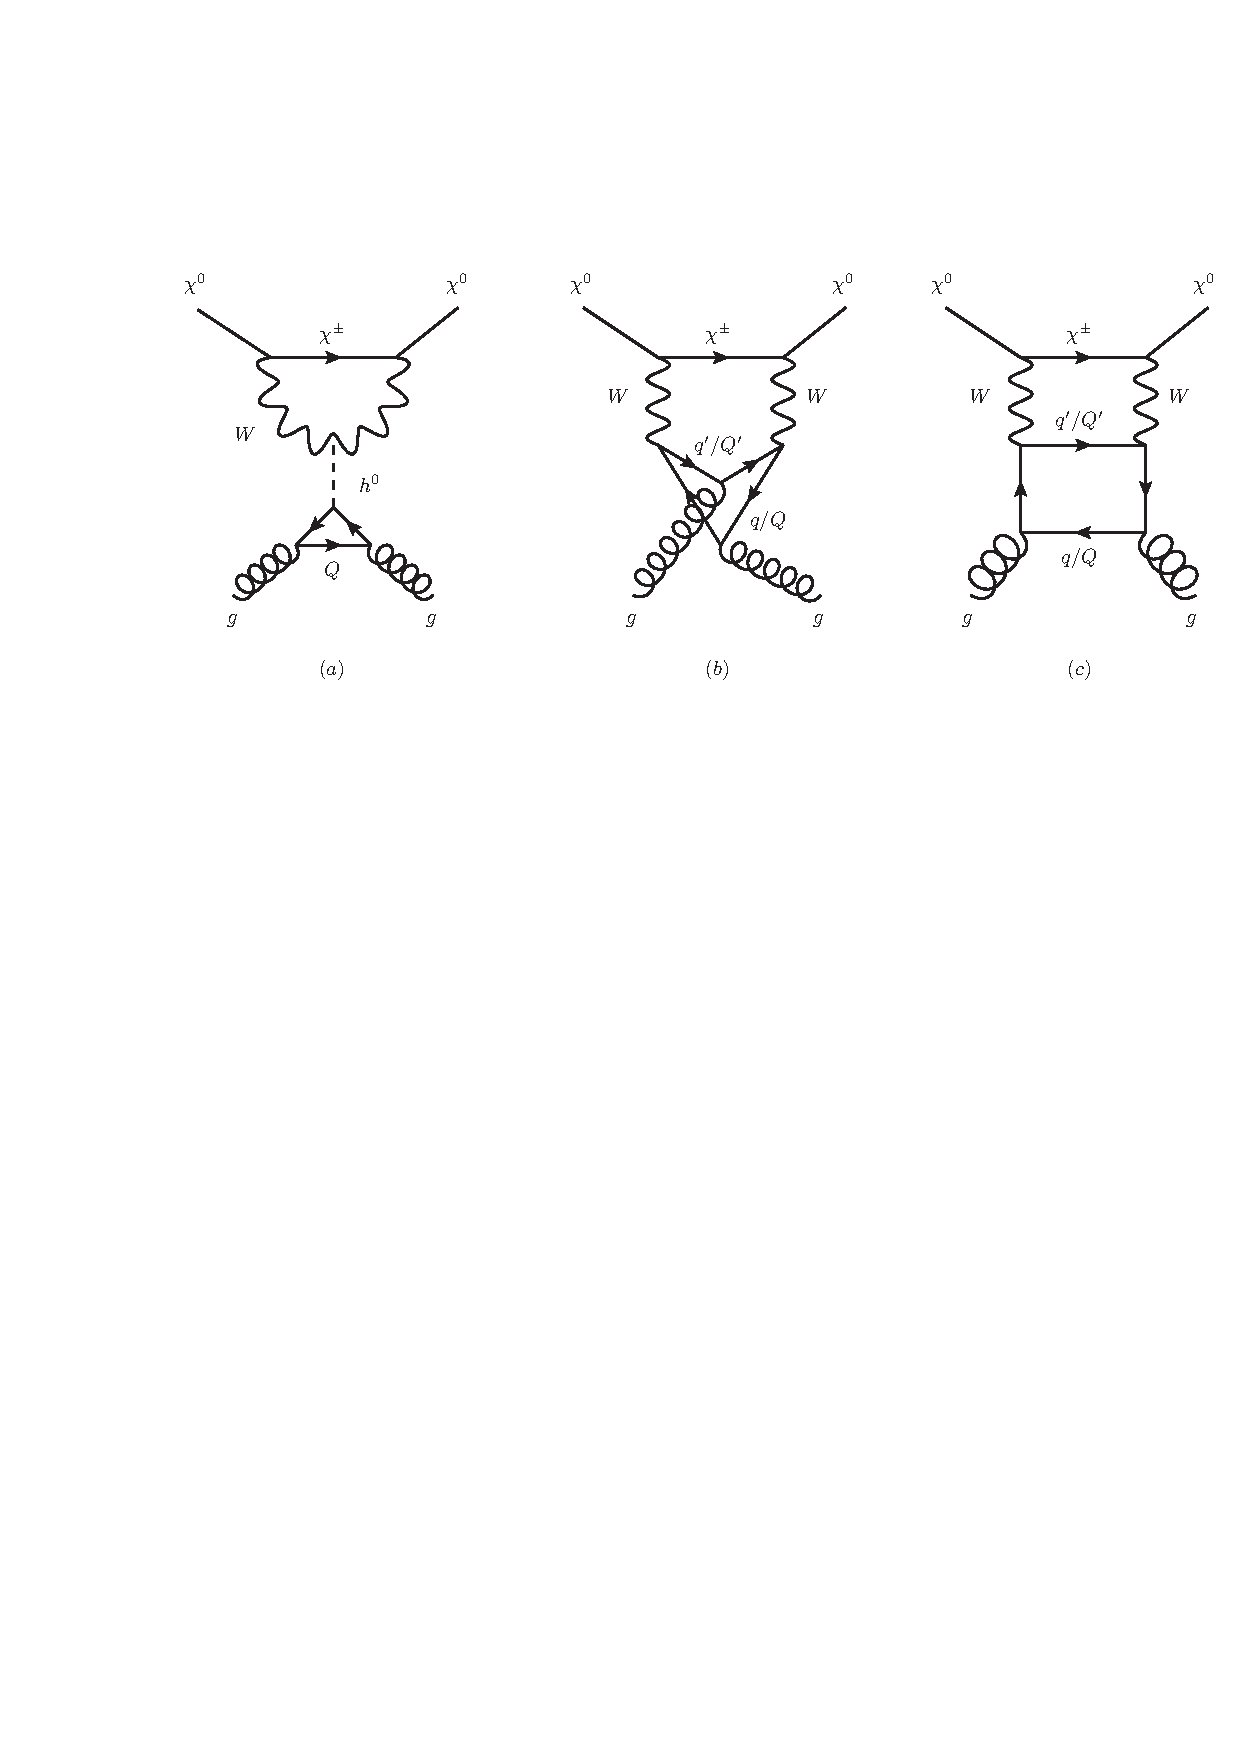
\includegraphics[width=1\textwidth]{../pics/gluon2loopB.pdf}
 \caption{Two loop diagrams contributing to the effective gluonic coupling.}
 \label{pic_2loopgluon}
\end{figure}
For the effective $\chi^0$-$q$-coupling follows
\begin{align}
 f_q =& \frac{\alpha_2^2}{4m_W m_{h}^2} g_H(w),\\
 g^{(1)}_q =& \frac{\alpha_2^2}{m_W^3}g_{T1}(w),\\
 g^{(2)}_q =&\frac{\alpha_2^2}{m_W^3}g_{T2}(w), 
\end{align}
where $f_q$ gets its contributions from $h^0$ exchange and the $W$-box leads to $g^{(i)}_q$. The $W$-mass and the Higgs-mass are denoted by$m_W$ and 
$m_h$, respectively. The function argument is $w=\sfrac{m_W^2}{m_\chi^2}$ \\
\noindent Concerning the gluonic coupling, there are three dominating two loop processes, one via Higgs exchange (fig. \ref{pic_2loopgluon}a) and two
via $W$-boxes (fig. \ref{pic_2loopgluon}b, c). The first one is evaluated by comparing it to the effective quark coupling from figure \ref{pic_wloop}a
by exchanging the light scattered quarks with heavy loop quarks which hence contributes to the long distance interaction. 
The calculation of the other two diagrams is quite extensive since the loops have to be calculated explicitly with the additional treatment of the vacuum 
polarisation tensor of the $W$ \cite{1007.2601}. In the end we have for the effective $\chi^0$-$g$ coupling reads
\begin{align}
 f_G = \frac{\alpha_s\alpha_2^2}{4\pi m_W}\left(-\sum\limits_Q c_Q \frac{1}{3m_{h^0}^2} g_H(w) + \frac{1}{m_W^2} g_{W}(w,t) \right)
\end{align}
with $t=\sfrac{m_t^2}{m_\chi^2}$ ($m_t$ is the top mass).
With the additional scalar $\chi^0$-$q$ coupling giving a contribution to the form factor as $\sum_qf_{Tq}f_q$, the result is
\begin{align}
 \frac{f_N}{m_N} &= \frac{\alpha_2^2}{m_W^3}\left(\sum\limits_{q,c,b} \frac34 \left(q(2)+\bar q(2)\right) \left(g_{T1}(w) + g_{T2}(w)\right) + \frac29g_W(w,t)\right) \\
 \nonumber
 &+ \frac{\alpha_2^2}{m_W m_h^2}g_H(w) \left(\frac14 \sum\limits_q f_{Tq} - \frac{2}{27}f_{TG}\sum\limits_Q c_Q \right).
\end{align}
As stated in the beginning of this section, the cross section only depends
on $m_\chi$. The mass difference of the charged triplet components to the neutral one is assumed to be negligable compared to the mass scale itself,
so they do not enter explicitly. 

% \begin{align}
%  \sigma_\text{SI} = \frac{4}{\pi}\mu_N^2 \left| f_N \right| ^2 \approx 4.57\cdot 10^{-18} \mu_N^2 \cdot \left(0.51 \left(g_{T1}+g_{T2}\right) + \frac29 g_W - 0.02 g_H\right)
%  \label{eq_sigmaDDB}
% \end{align}
% with the masses in GeV. Unlike \eqref{eq_sigmaDDA} the cross section for the triplet case only depends on the DM mass which makes it generally very
% interesting in constraining such models. 













\subsection{DM Annihilation}
\begin{figure}[t]
 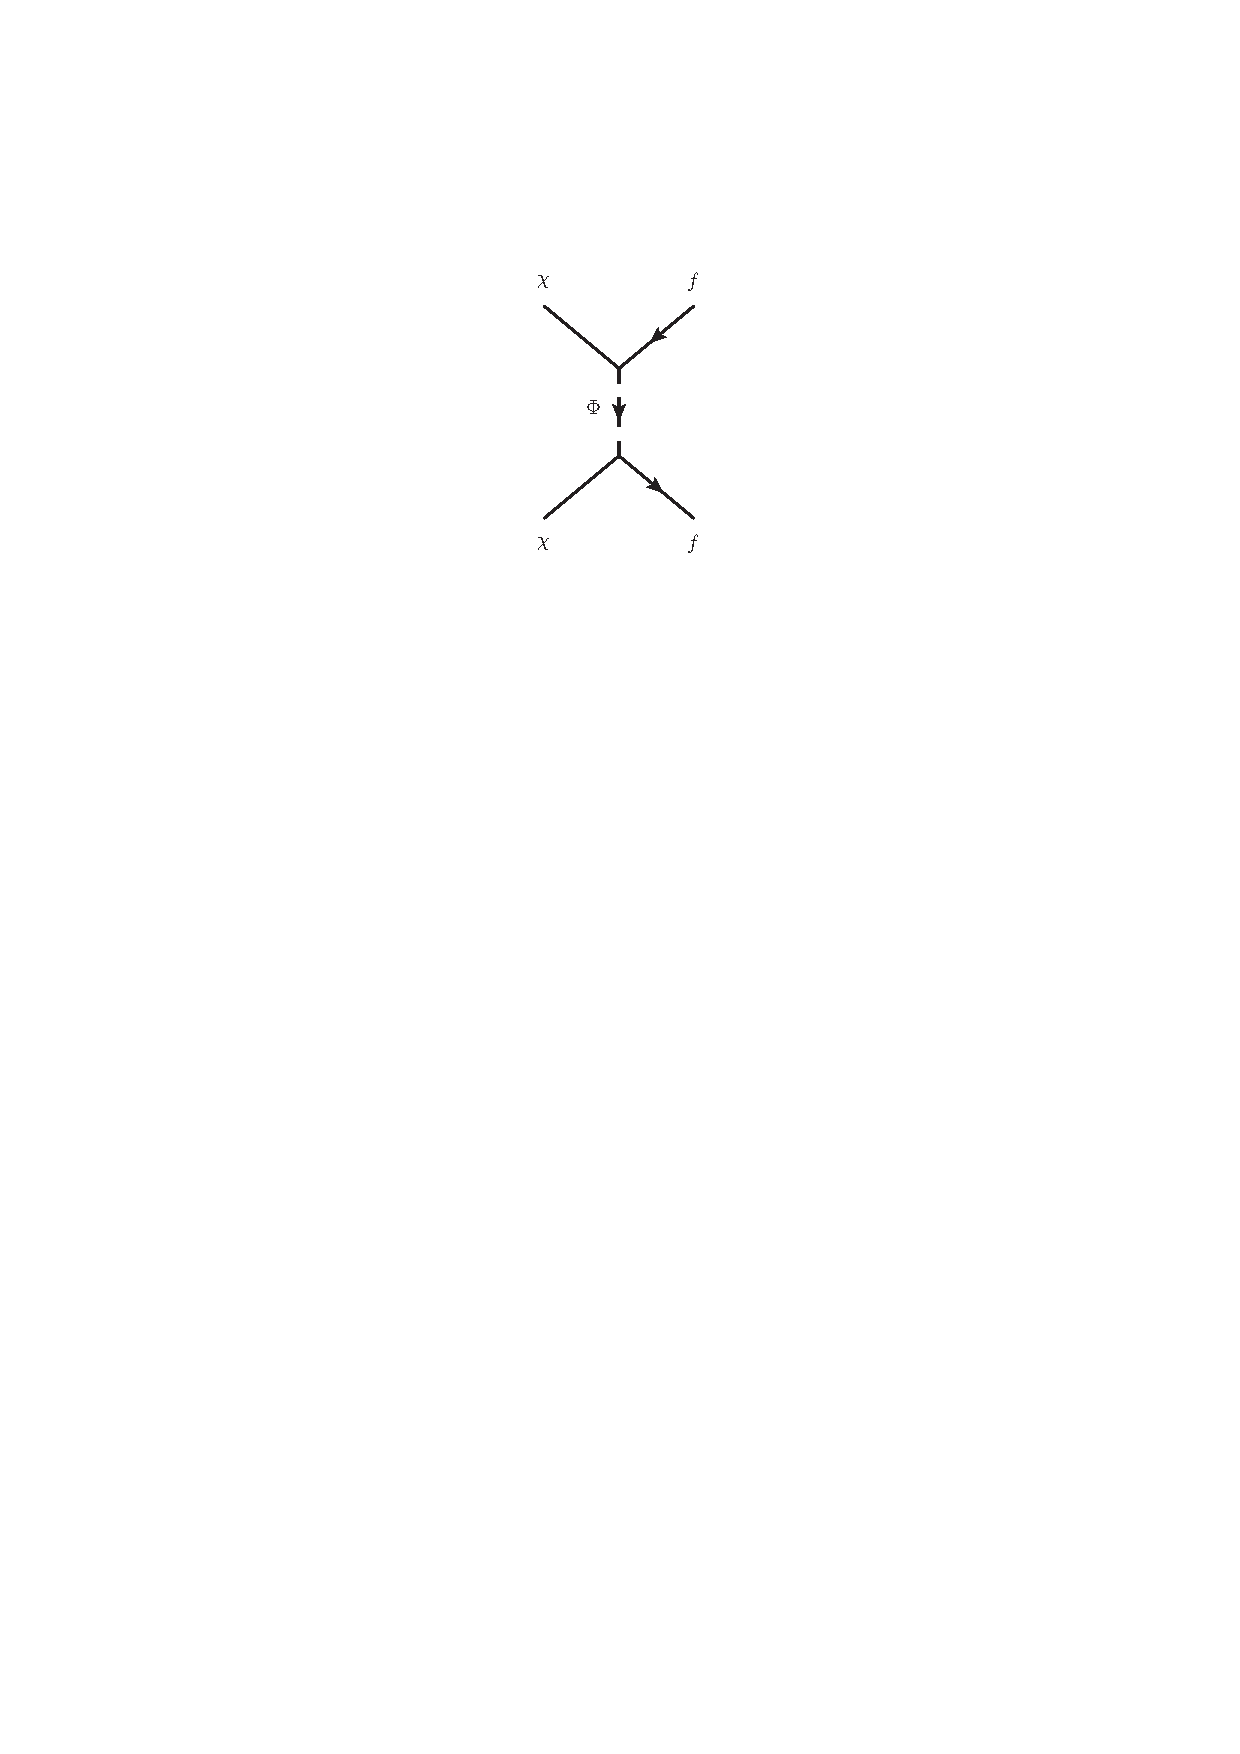
\includegraphics[width=0.3\textwidth]{../pics/ann.pdf}
 \caption{Annihilation process.}
 \label{pic_annihilation}
\end{figure}
% $VV$ annihilation (9207234), wino RD from other su2-states (0913-main)
% \begin{align}
%  \langle \sigma v \rangle^\text{D} \left(\bar \chi \chi \rightarrow \bar f f\right) = \frac{N_c g_f^4 m^2}{32\pi^2\left(M_l^2 + m^2\right)^2}
% \end{align}
The leading contribution for annihilation cross section for $\bar\chi^0 \chi^0 \rightarrow \bar f f$ (fig. \ref{pic_annihilation} is for both representations (1506.03116)
\begin{align}
 \langle \sigma v \rangle^\text{M} \left(\bar \chi \chi \rightarrow \bar f f\right) = \frac{N_c g_f^4 m^2 \left(M^4+m^4 \right)}{48\pi^2\left(M_l^2 + m^2\right)^4}v^2.
\end{align}
No co-annihilations are considered here for assumed non-degeneracy of the fermion and scalar masses. $v\approx 0.3$ during freeze-out. Nowadays 
$2\rightarrow3$ processes as $\bar \chi \chi \rightarrow \bar f f V$ might dominate with lower velocities $v\approx 10^{-3}$, interesting for 
indirect detection (1207.1431). 
% 
% \begin{align}
%  \text{cm}^2 = 2.57e27 1/GeV^2\\
%  \text{cm}^3/\text{s} = 7.70e17 1/GeV^2\\
%  \text{pb} = 2.57e-8 1/GeV^2
% \end{align}


\section{Results}
% supersymmetry
The used parameters for the following plots are
\begin{align}
 |g^l_2| &= 2\\
 |g^q_2| &= 0.04\\
 |g^q_3| &= 1\\
 M_{\Phi_l} &= m_\chi + 200 GeV\\
 M_{\Phi_q} &= m_\chi + 800 GeV\\
 \label{eq_resParams}
\end{align}

\subsection{A - $T(\chi)=\boldsymbol{1}$}
% binolike
\textit{$B_s$ Processes}\\
\noindent \ref{pic_BsResA}
\begin{figure}[t]
 \includegraphics[width=1\textwidth]{../pics/BsModA.pdf}
 \caption{Paramter space plot for $B_s$ mixing and $B_s\rightarrow \mu\mu$.}
 \label{pic_BsResA}
\end{figure}
\\ \textit{Anomalous Magnetic Moment of the Muon}\\
\noindent \ref{pic_g-2A}
\begin{figure}[t]
 \includegraphics[width=1\textwidth]{../pics/g-2A.pdf}
 \caption{Paramter space plot for anomalous magnetic moment of the muon. The area of the blue line crossing the higher and lower bound is valid.}
 \label{pic_g-2A}
\end{figure}

\subsection{B - $T(\chi)=\boldsymbol{3}$}
%winolike
\textit{$B_s$ Processes}\\
\noindent \ref{pic_BsResB}
\begin{figure}[t]
 \includegraphics[width=1\textwidth]{../pics/BsModB.pdf}
 \caption{Paramter space plot for $B_s$ mixing and $B_s\rightarrow \mu\mu$.}
 \label{pic_BsResB}
\end{figure}
\\ \textit{Anomalous Magnetic Moment of the Muon}\\
\noindent \ref{pic_g-2B}
\begin{figure}[t]
 \includegraphics[width=1\textwidth]{../pics/g-2B.pdf}
 \caption{Paramter space plot for anomalous magnetic moment of the muon. The area of the blue line crossing the higher and lower bound is valid.}
 \label{pic_g-2B}
\end{figure}
\\ \textit{Direct Detection} \\
\noindent \ref{pic_ddB}
\begin{figure}[t]
 \includegraphics[width=1\textwidth]{../pics/ddB.pdf}
 \caption{Paramter space plot for nucleon scattering. The cross section for the triplet is barely below current bounds and will be tested next year.}
 \label{pic_ddB}
\end{figure}
\\ \textit{Annihilation}\\
With \eqref{eq_resParams} there are two masses for which $m_\chi$ as a thermal relic makes up for all DM in universe. They are 80 and 350 GeV. In
between the cross section is too high leaving the DM candidate over abundant. Its peak is around 120 GeV.


\section{Conclusion and Prospects}

% dfasdölkj\\d\\d\\d\\d\\d\\d\\d\\d\\d\\d\\d

% \section{DM candidate coupling to light quarks in T' framework}
% \subsection{Model construction}
% % \subsubsection{Grouptheoretical properties}
% \begin{align}
%  \sum m_n n^2 = N_G \quad groupelements\\
%  \sum m_n = \#_{IRR} \quad C = Irred\,Reps\\
%  \varphi:\, G\rightarrow \text{GL}(V)\\
%  g\mapsto \varphi(g):\, V\rightarrow V\\
%  \chi_D(g) = \text{tr}D(g)\\
%  \sum_g \chi_\alpha(g)^*\chi_\beta(g) = N_G \delta_{\alpha\beta}\\
%  \sum_\alpha \chi_\alpha(g)^*\chi_\alpha(h) = \frac{N_G}{n_g} \delta_{C_g C_h} \stackrel{\Lambda}{=} \langle \chi^\mu, \chi^\nu \rangle = \delta^{\mu\nu}\\
%  \text{FS}(R) := \frac{1}{N_G} \sum_g \chi_R(g^2) =\begin{cases}
%                                                     1, & \text{real}\\
%                                                     0, & \text{complex}\\
%                                                     -1, & \text{pseudoreal}\\
%                                                    \end{cases}\\
%  \mu(k) = \langle \chi_R \cdot \chi_{R'} , \chi_{R_k} \rangle \quad tensor product decomposation\\
% \end{align}
% 
% \subsubsection{Assigning particles to multiplets}
% \begin{align}
%  \langle \xi'' \rangle = \delta u''\approx \epsilon^4 \Lambda\\
%  M_{\xi''} = k \delta u'' 
% \end{align}
% 
% \subsection{Messenger $\xi''$ mediating SM and DM}
% \subsubsection{DM annihilation into light mesons}
% \subsubsection*{DM stability}
% page 24 - check on T, Z3 reps and spin
% \subsubsection*{cross section}
% \begin{align}
%  \sigma(\chi\chi \rightarrow d \bar s) = \frac{\lambda_f^2\lambda_\chi^2}{8\pi(4m_\chi^2 - M_{\xi''}^2)^2}(4m_\chi^2 - (m_d+m_s)^2)\\
%  \langle \sigma_{\text{Ann}} v \rangle = \sigma(1+\frac18
% \end{align}
% 
% \subsubsection{Meson-Mixing}
% \begin{align}
%  \Xi_{dd'} = \begin{pmatrix}
%               0 & 1 & 0\\
%               1 & 0 & 0 \\
%               0 & 0 & 0
%              \end{pmatrix} \xrightarrow{massbasis} \begin{pmatrix}
% 						-\epsilon & 1 & -\epsilon^2\\
% 						1 & \epsilon & -\epsilon^3\\
% 						-\epsilon^2 & \-\epsilon^3 & \epsilon^5
% 						\end{pmatrix}
% \end{align}
% 
% \subsubsection{DM-nucleus scattering}
% 
% 
% \addcontentsline{toc}{section}{List of figures}
% \newpage\listoffigures\newpage
% \addcontentsline{toc}{section}{List of tables}
% \listoftables\newpage
\end{spacing}
\newpage

\begin{thebibliography}{xxx}
 \bibitem[1]{Grip}B. Gripaios et al. \textit{Linear flavour violation and anomalies in $B$ physics} \href{http://arxiv.org/abs/1509.05020v1}{arxiv.org/abs/1509.05020v1}
 \bibitem[2]{Peskin}M. Peskin et al. \textit{An Introduction To Quantum Field Theory} ISBN: 0-201-50397-2
 \bibitem[3]{Fierz}J.F. Nieves et al. \textit{Generalized Fierz identities} \href{http://arxiv.org/abs/hep-ph/0306087v1}{arxiv.org/abs/hep-ph/0306087v1}
 \bibitem[4]{FerA4}G. Altarelli et al. \textit{Tri-Bimaximal Neutrino Mixing and Discrete Flavour Symmetries} \href{https://arxiv.org/abs/1205.5133}{arxiv.org/abs/1205.5133}
 \bibitem[5]{VarzTotMod}I.d.M. Varzielas et al. \textit{Clues for flavour from rare lepton and quark decays} \href{https://arxiv.org/abs/1503.01084}{arxiv.org/abs/1503.01084}
 \bibitem[6]{Hisano}J. Hisano et al. \textit{Direct Detection of Electroweak-Interacting Dark Matter} \href{https://arxiv.org/abs/1104.0228v2}{arxiv.org/abs/1104.0228v2}
 \bibitem[7]{minMatter}E.D. Nobile et al. \textit{Minimal Matter at the Large Hadron Collider} \href{http://arxiv.org/abs/0908.1567}{arxiv.org/abs/0908.1567}
 \bibitem[8]{anomMom}K. Melnikov et al. \textit{Theory of the Muon Anomalous Magnetic Moment} ISBN-13 978-3-540-32806-3
 \bibitem[9]{Lavoura}L. Lavoura \textit{General formulae for $f_1\rightarrow f_2 \gamma$} \href{http://arxiv.org/abs/hep-ph/0302221}{arxiv.org/abs/hep-ph/0302221}
 \bibitem[10]{BurasEFT}A.J. Buras \textit{Weak Hamiltonian, CP Violation and Rare Decays} \href{http://arxiv.org/abs/hep-ph/9806471}{arxiv.org/abs/hep-ph/9806471}
 \bibitem[11]{LambdaCDM}P. Bull et al. \textit{Beyound $\Lambda$CDM: Problems, solutions, and the road ahead} \href{http://arxiv.org/abs/1512.05356}{arxiv.org/abs/1512.05356}
 \bibitem[12]{14041938}J.I. Read \textit{The Local Dark Matter Density} \href{http://arxiv.org/abs/1404.1938}{1404.1938}
 \bibitem[13]{LectDMLis}M. Lisanti \textit{Lectures on Dark Matter Physics} \href{https://arxiv.org/abs/1603.03797}{1603.03797}
 \bibitem[14]{160607790}A.D. Popolo et al.\textit{Small scale problems of the $\Lambda$CDM model: short review} \href{https://arxiv.org/abs/1606.07790}{1606.07790}
 \bibitem[15]{11015122}M. Milgrom \textit{MD or DM? Modified dynamics at low accelerations vs dark matter} \href{https://arxiv.org/abs/1101.5122}{1101.5122}
 \bibitem[16]{DM-EvCaDo}G. Bertone et al. \textit{Particle Dark Matter: Evidence, Candidates and Constraints}
\end{thebibliography}
\end{document}
